\documentclass[11pt,a4paper]{article}
\usepackage[utf8]{inputenc}
\usepackage{amsmath}
\usepackage{mathptm}
\usepackage{amsfonts}
\usepackage{amssymb}
\usepackage{graphicx}
\usepackage[a4paper]{geometry}
\usepackage[hyphens]{url}
\geometry{top=35mm, left=30mm, right=30mm, bottom=35mm}
\renewcommand{\contentsname}{Inhaltsverzeichnis}
\usepackage{graphicx}

\begin{document}
\begin{titlepage}
\begin{figure}
\centering
%\includegraphics[scale=5]{pics/2015_10_05_FHB_Logo_RGB_fbw.png}
\end{figure}
\title{Kali Linux Ausarbeitung}
\date{}

\maketitle
\end{titlepage}

\newpage
%\tableofcontents

\section {Installation von Linux Deploy auf Asus}
%\newpage

- Das Gerät muss gerootet sein \\
- Wir erhalten die Administrator-Rechte durch Super-SU

- Das folgende Bild zeigt die Schritte zu folgen:


%\begin{figure}
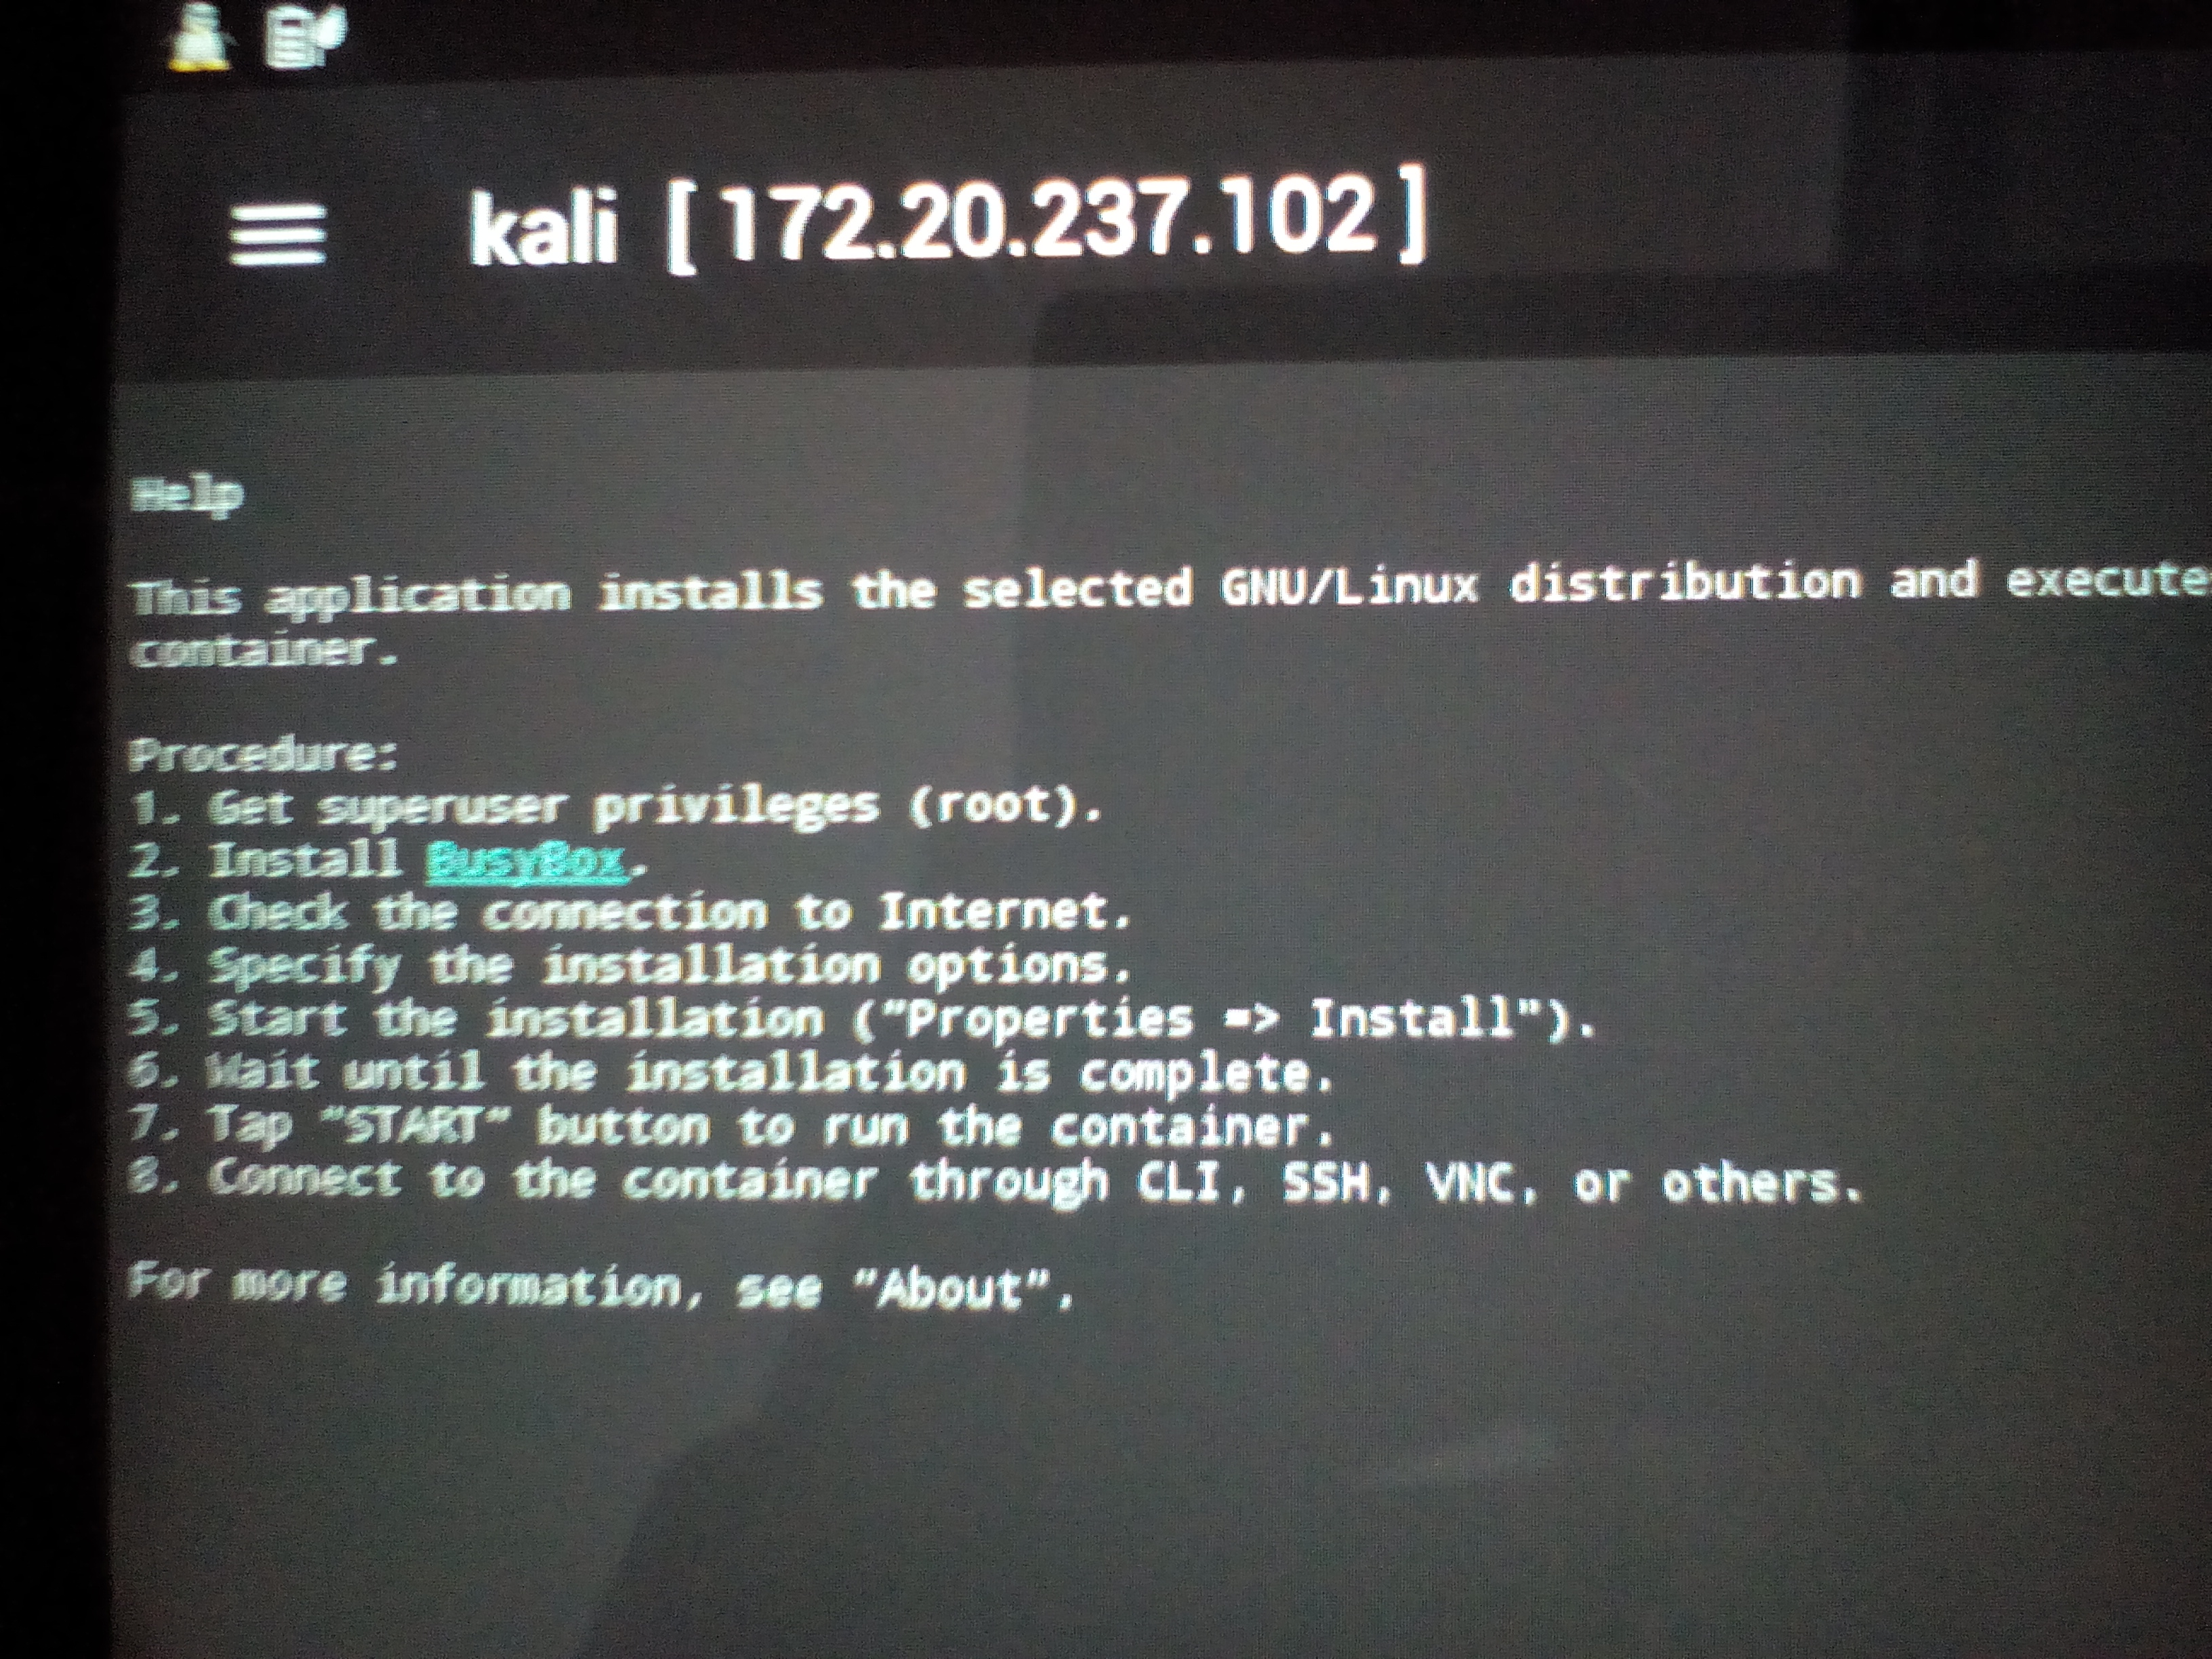
\includegraphics[scale=0.09]{./Image/img1} \\
%\caption{Schritte}
%\end{figure}

  
  Wir brauchen für die Installation: \\   
    
       \rule{1cm}{0cm}
\parbox{\linewidth}{    
	   - Die Virtuelle Maschine Busy Box \\
       - Linux Deploy \\
       - Android VNC Viewer \\ }
       
- Überprüfen, ob wir mit dem Internet verbunden sind \\
- Wir müssen auch die Parameter von Kali Linux Überprüfen \\ 
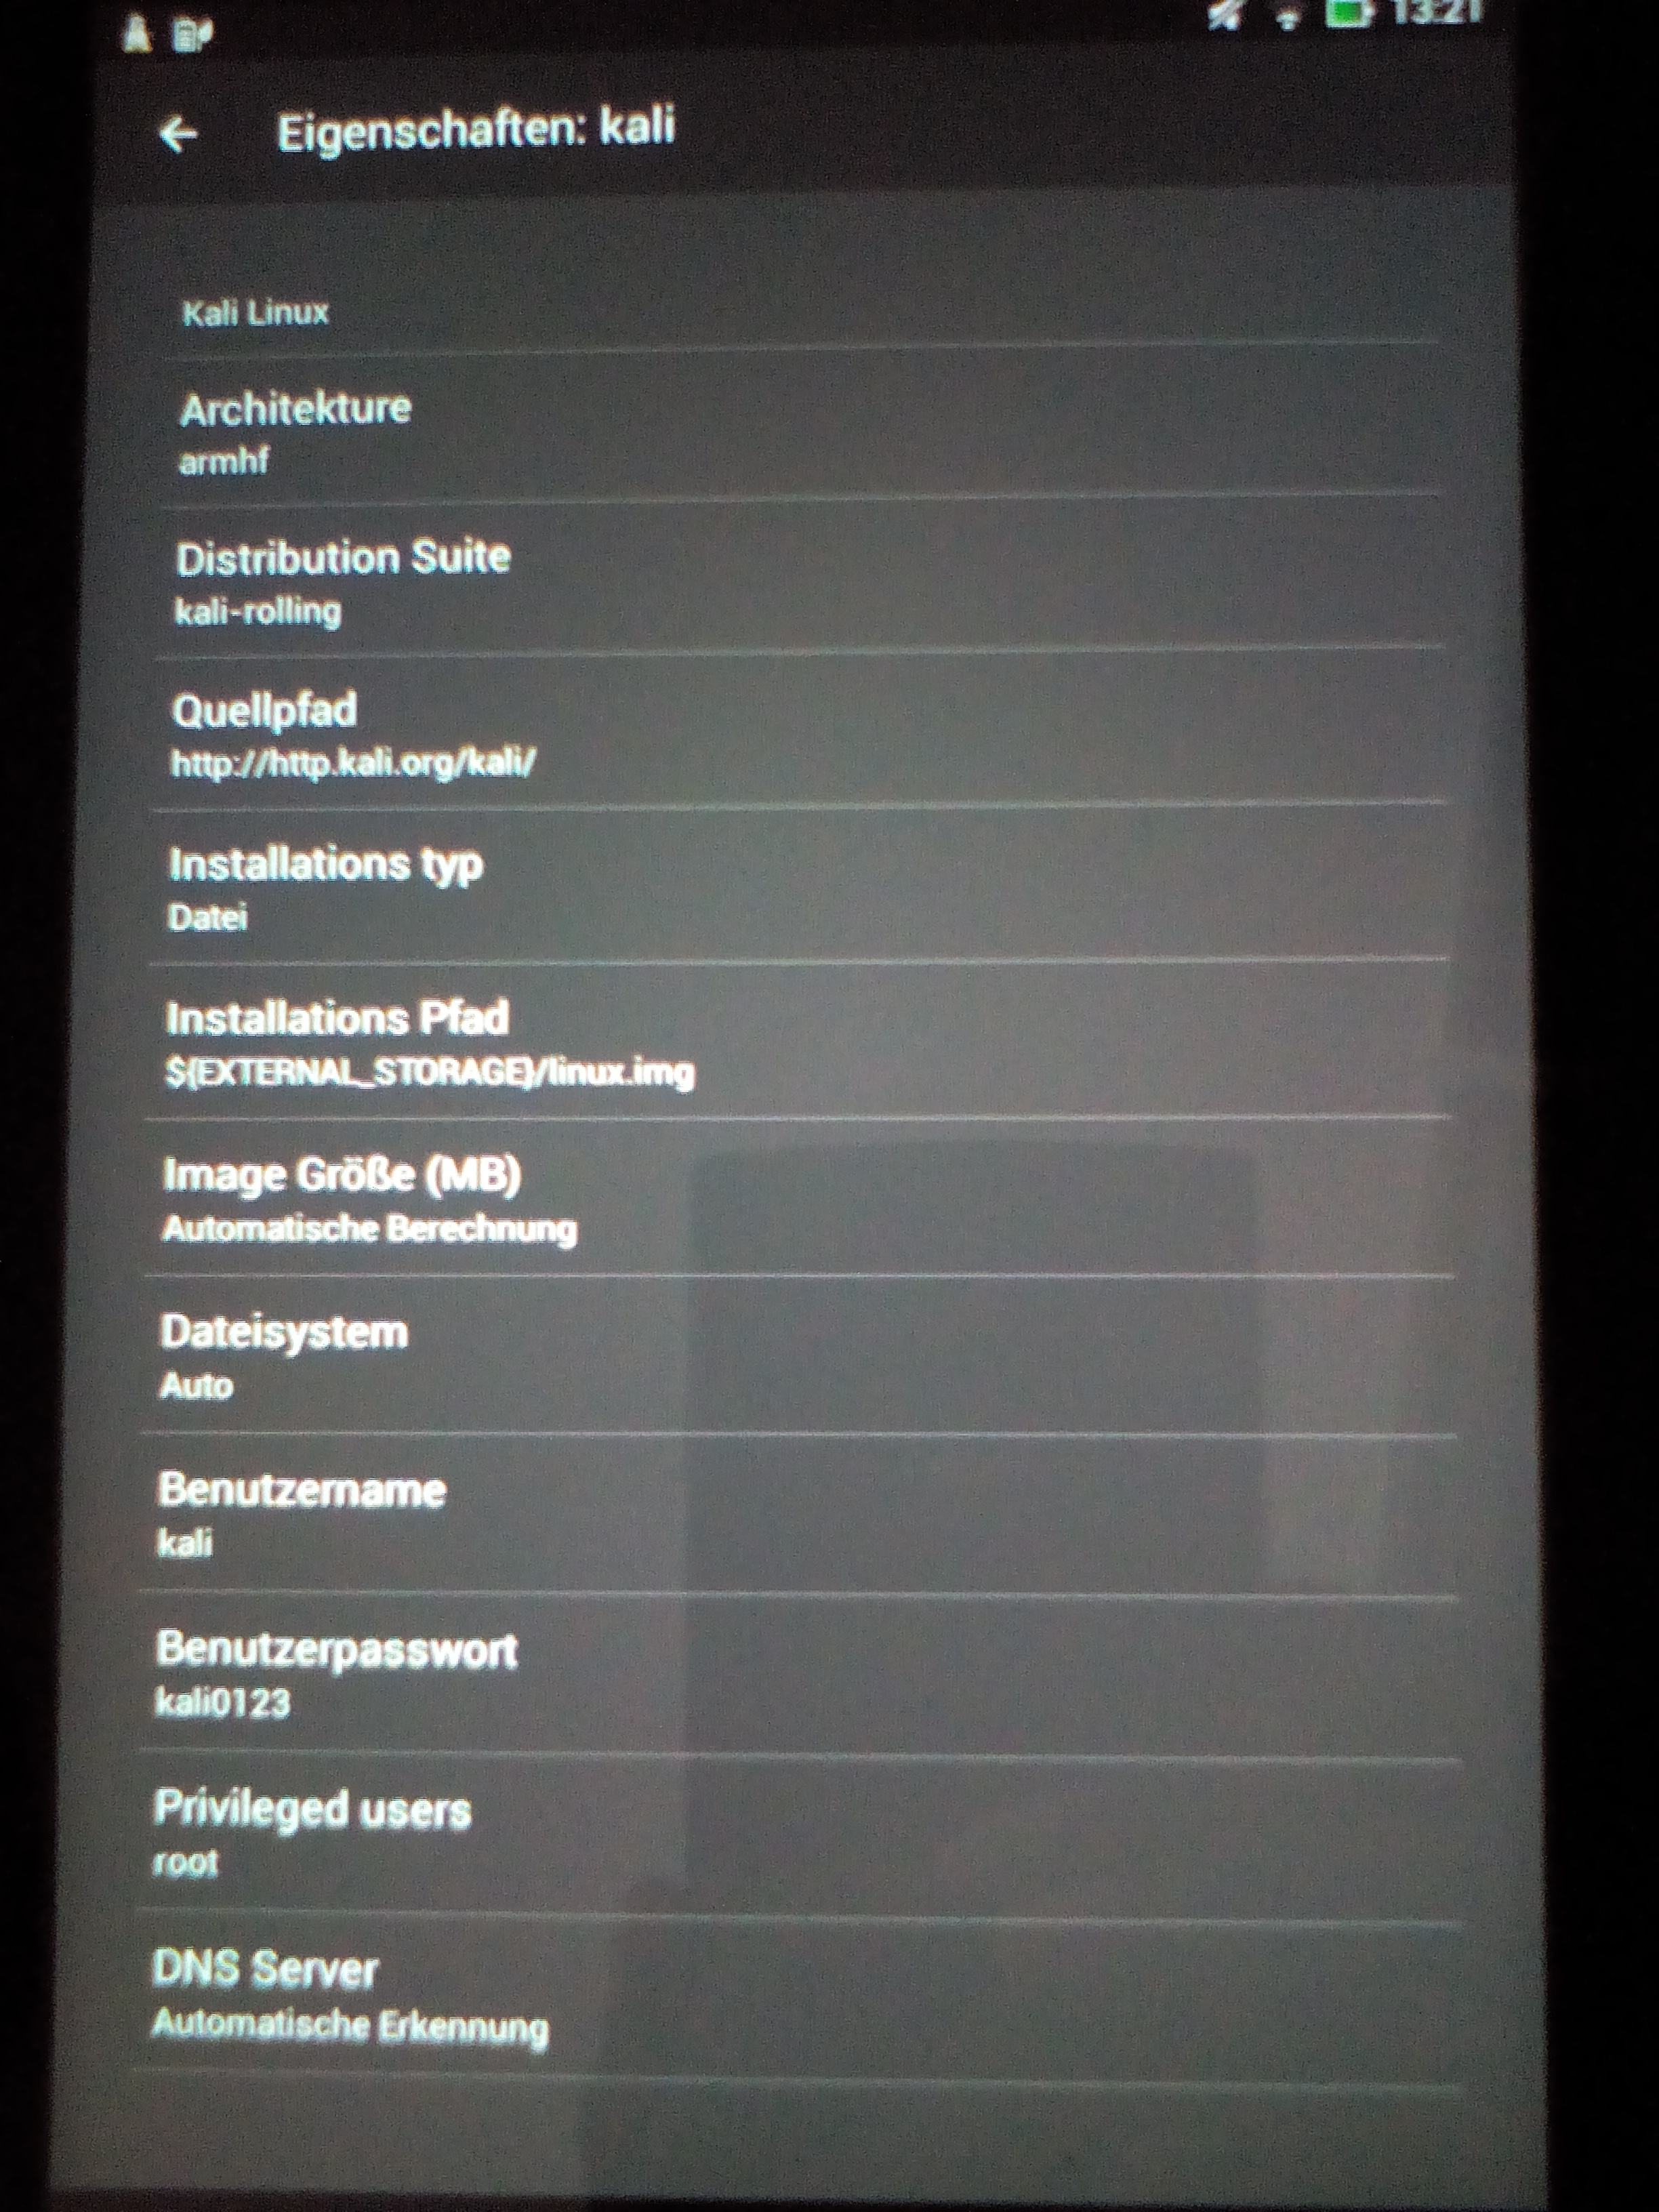
\includegraphics[scale=0.09]{./Image/img2} \\ \\
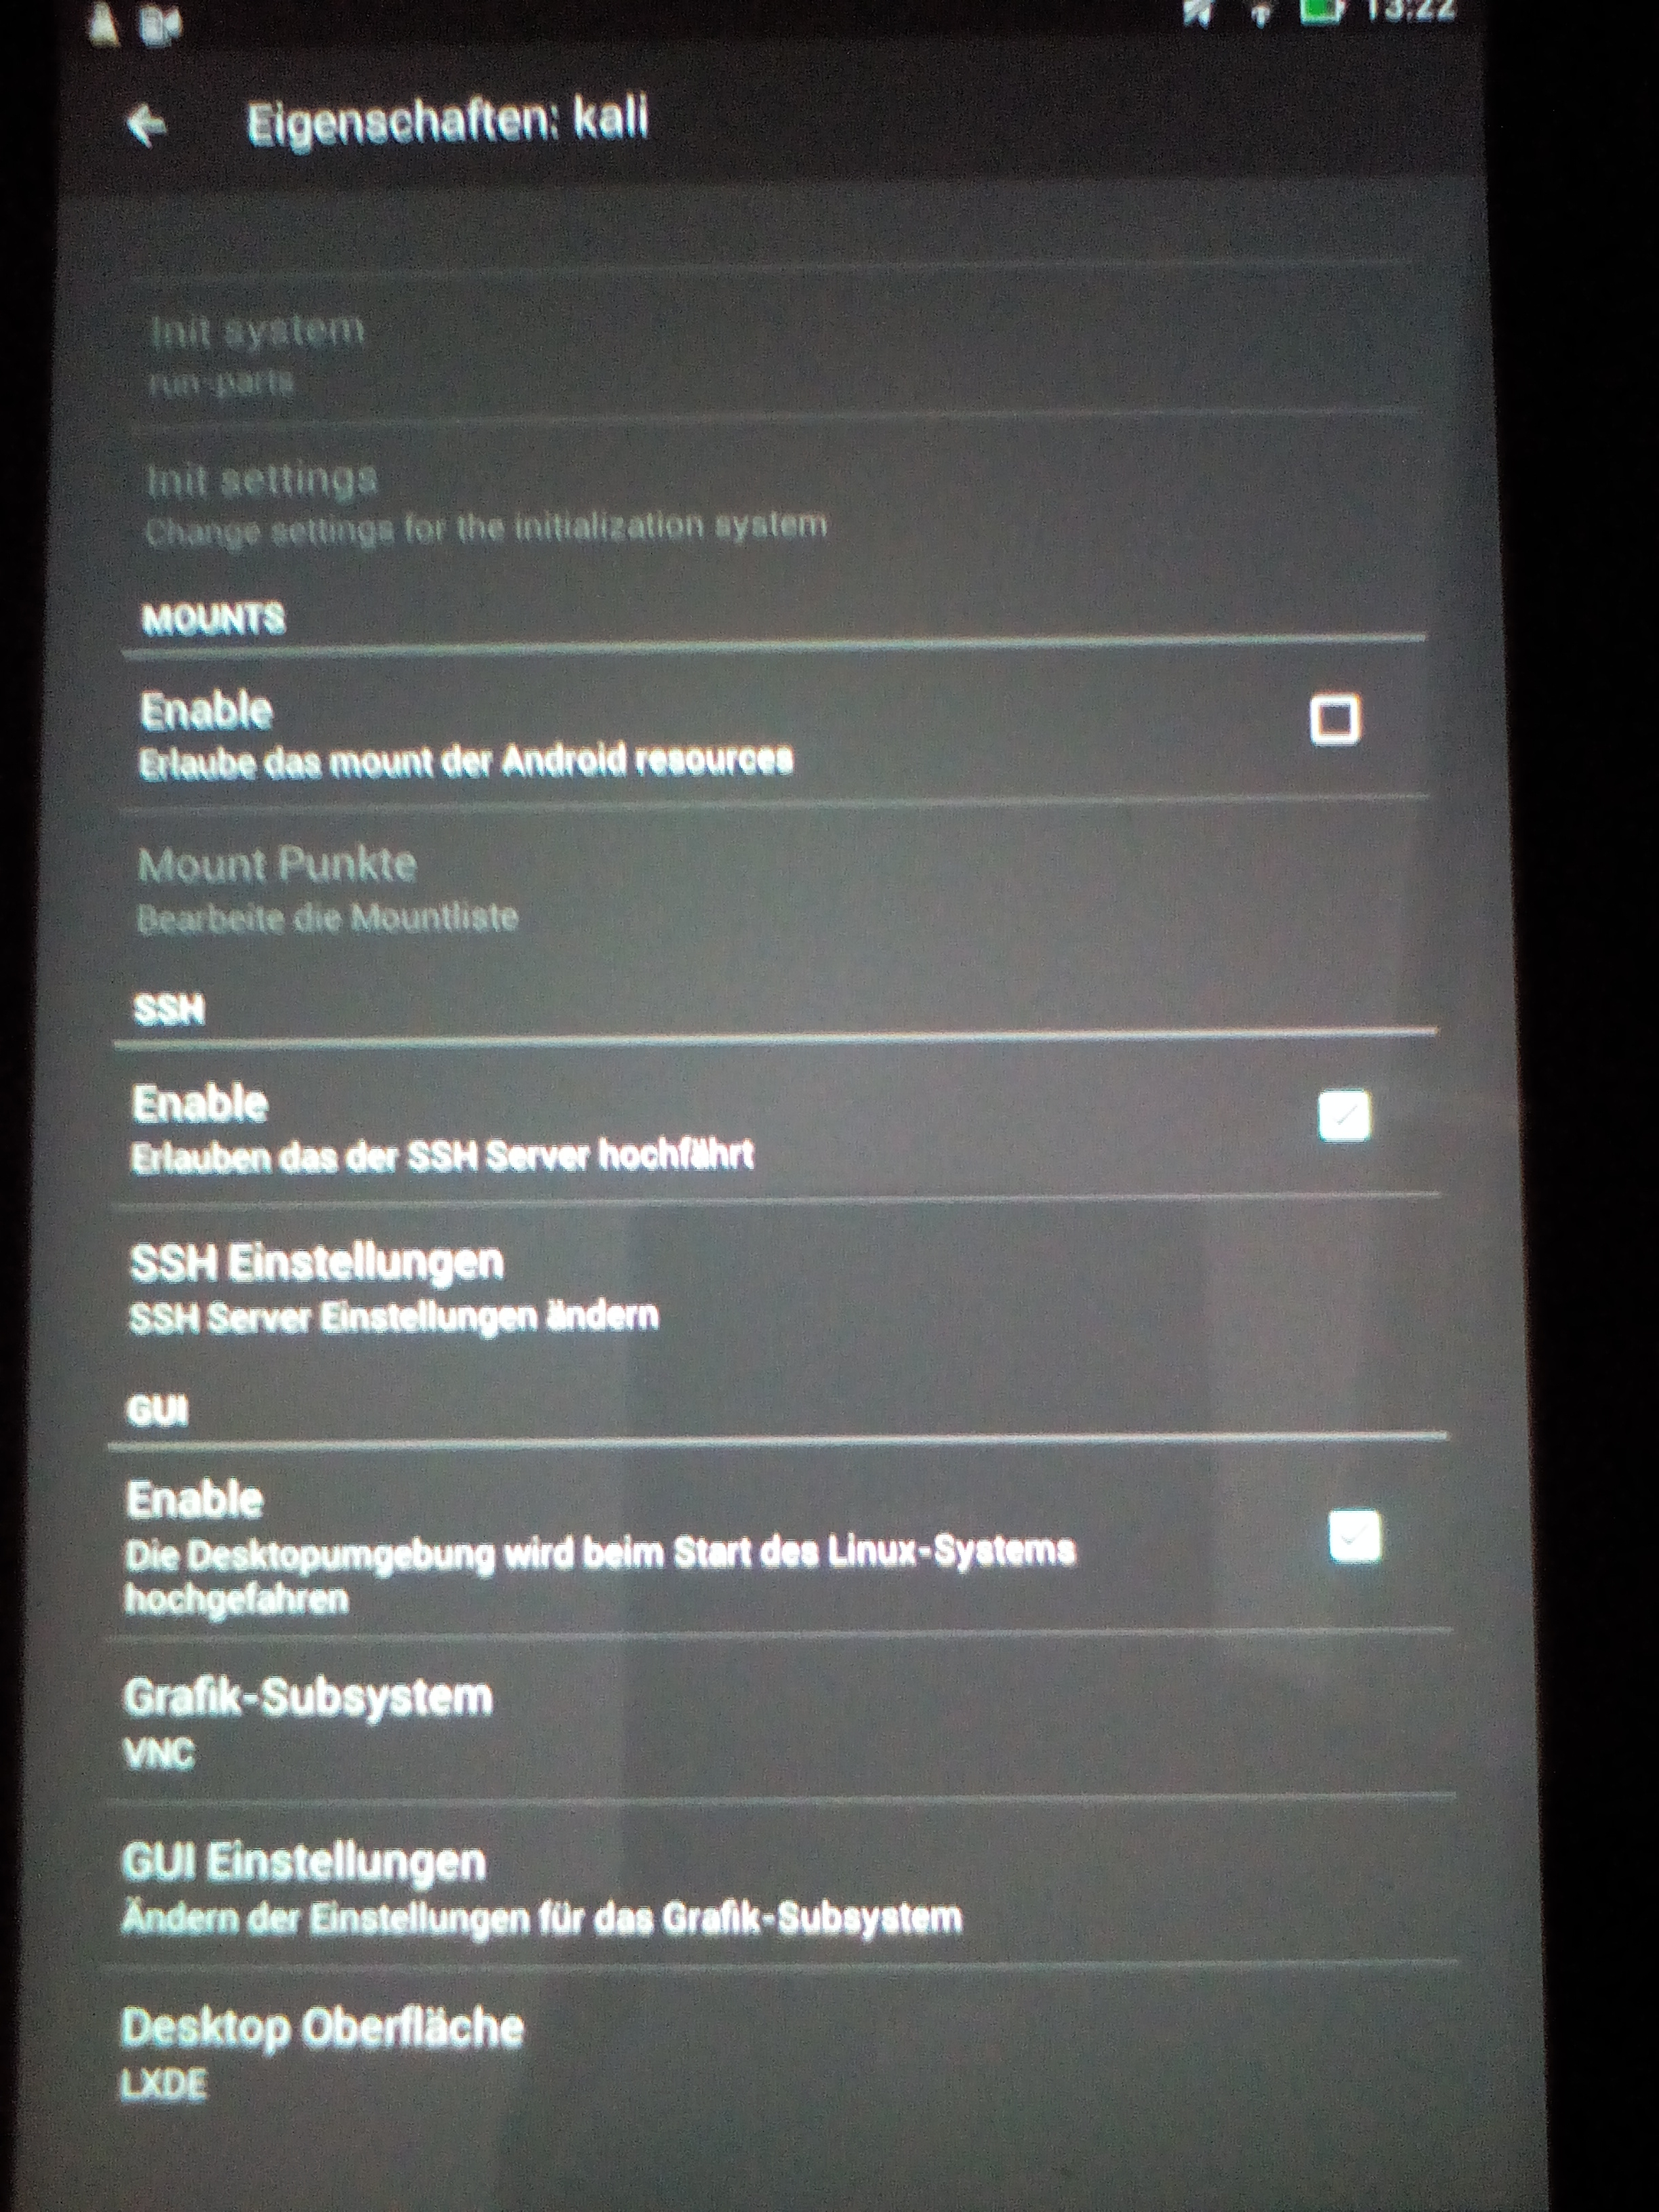
\includegraphics[scale=0.09]{./Image/img3} \\ \\

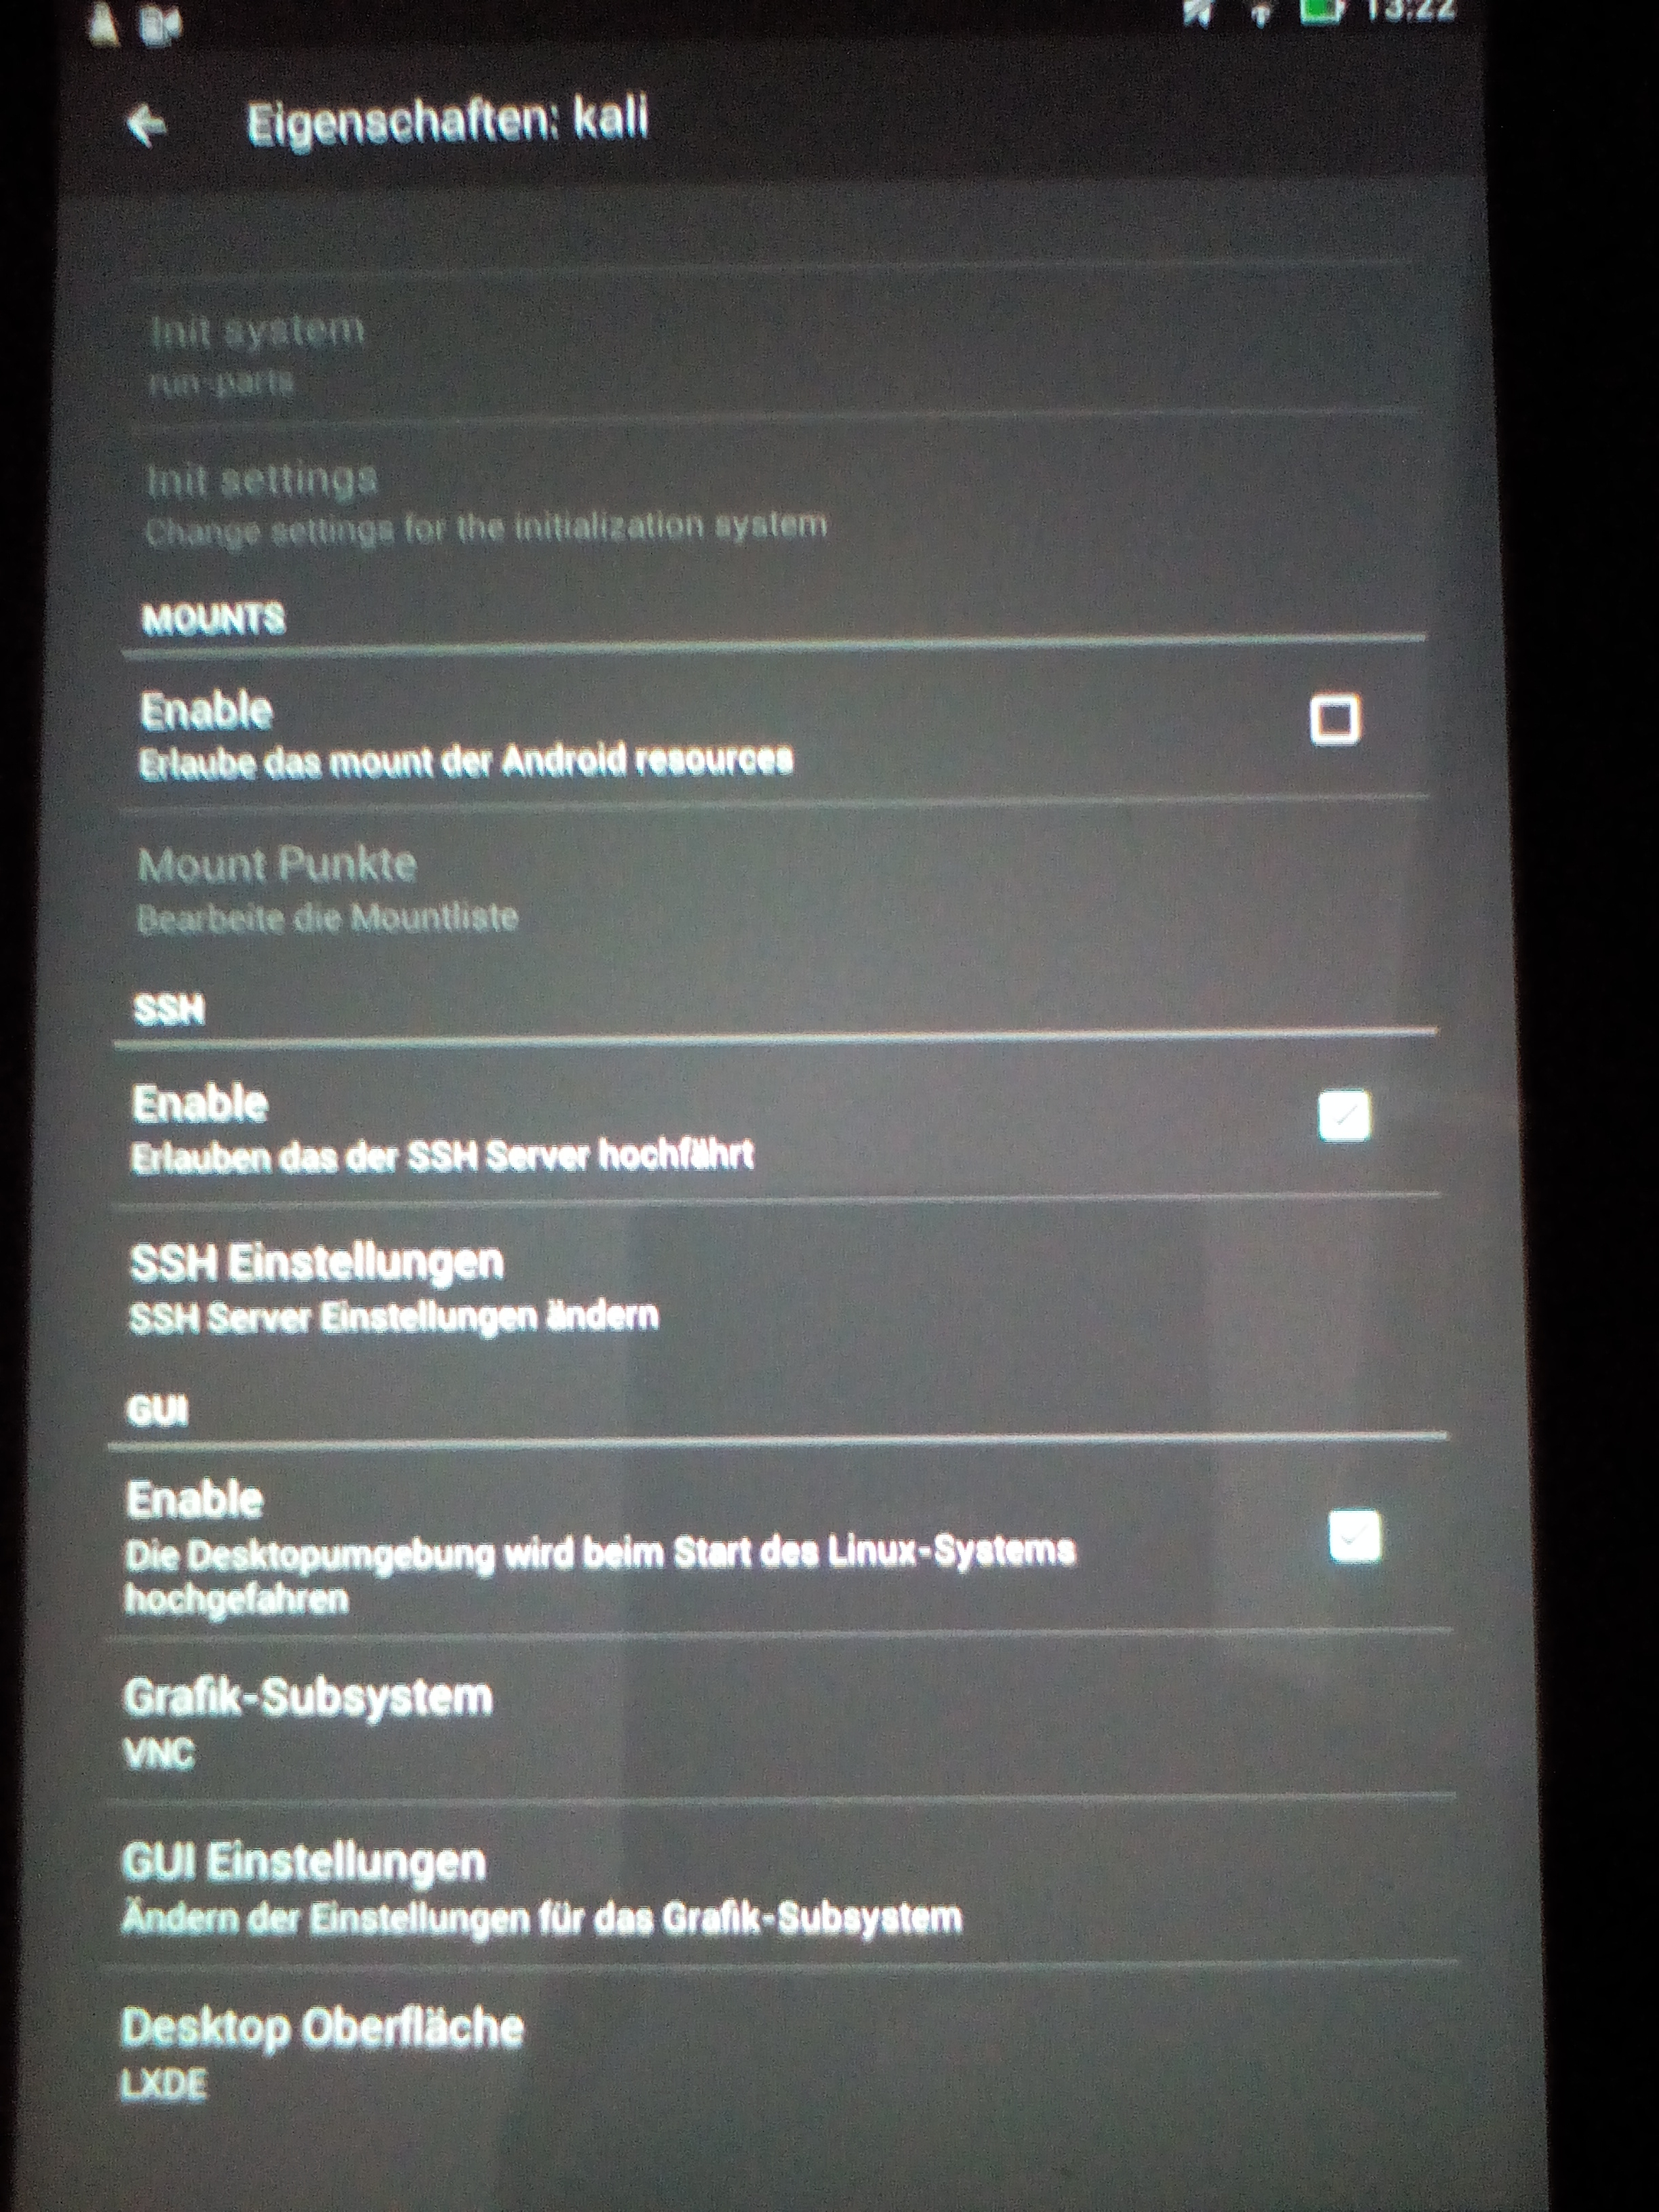
\includegraphics[scale=0.09]{./Image/img4} \\ \\
- Dann klicken wir auf "install" (Properties $\rightarrow$ Install) \\

- Dann klicken auf Configure \\
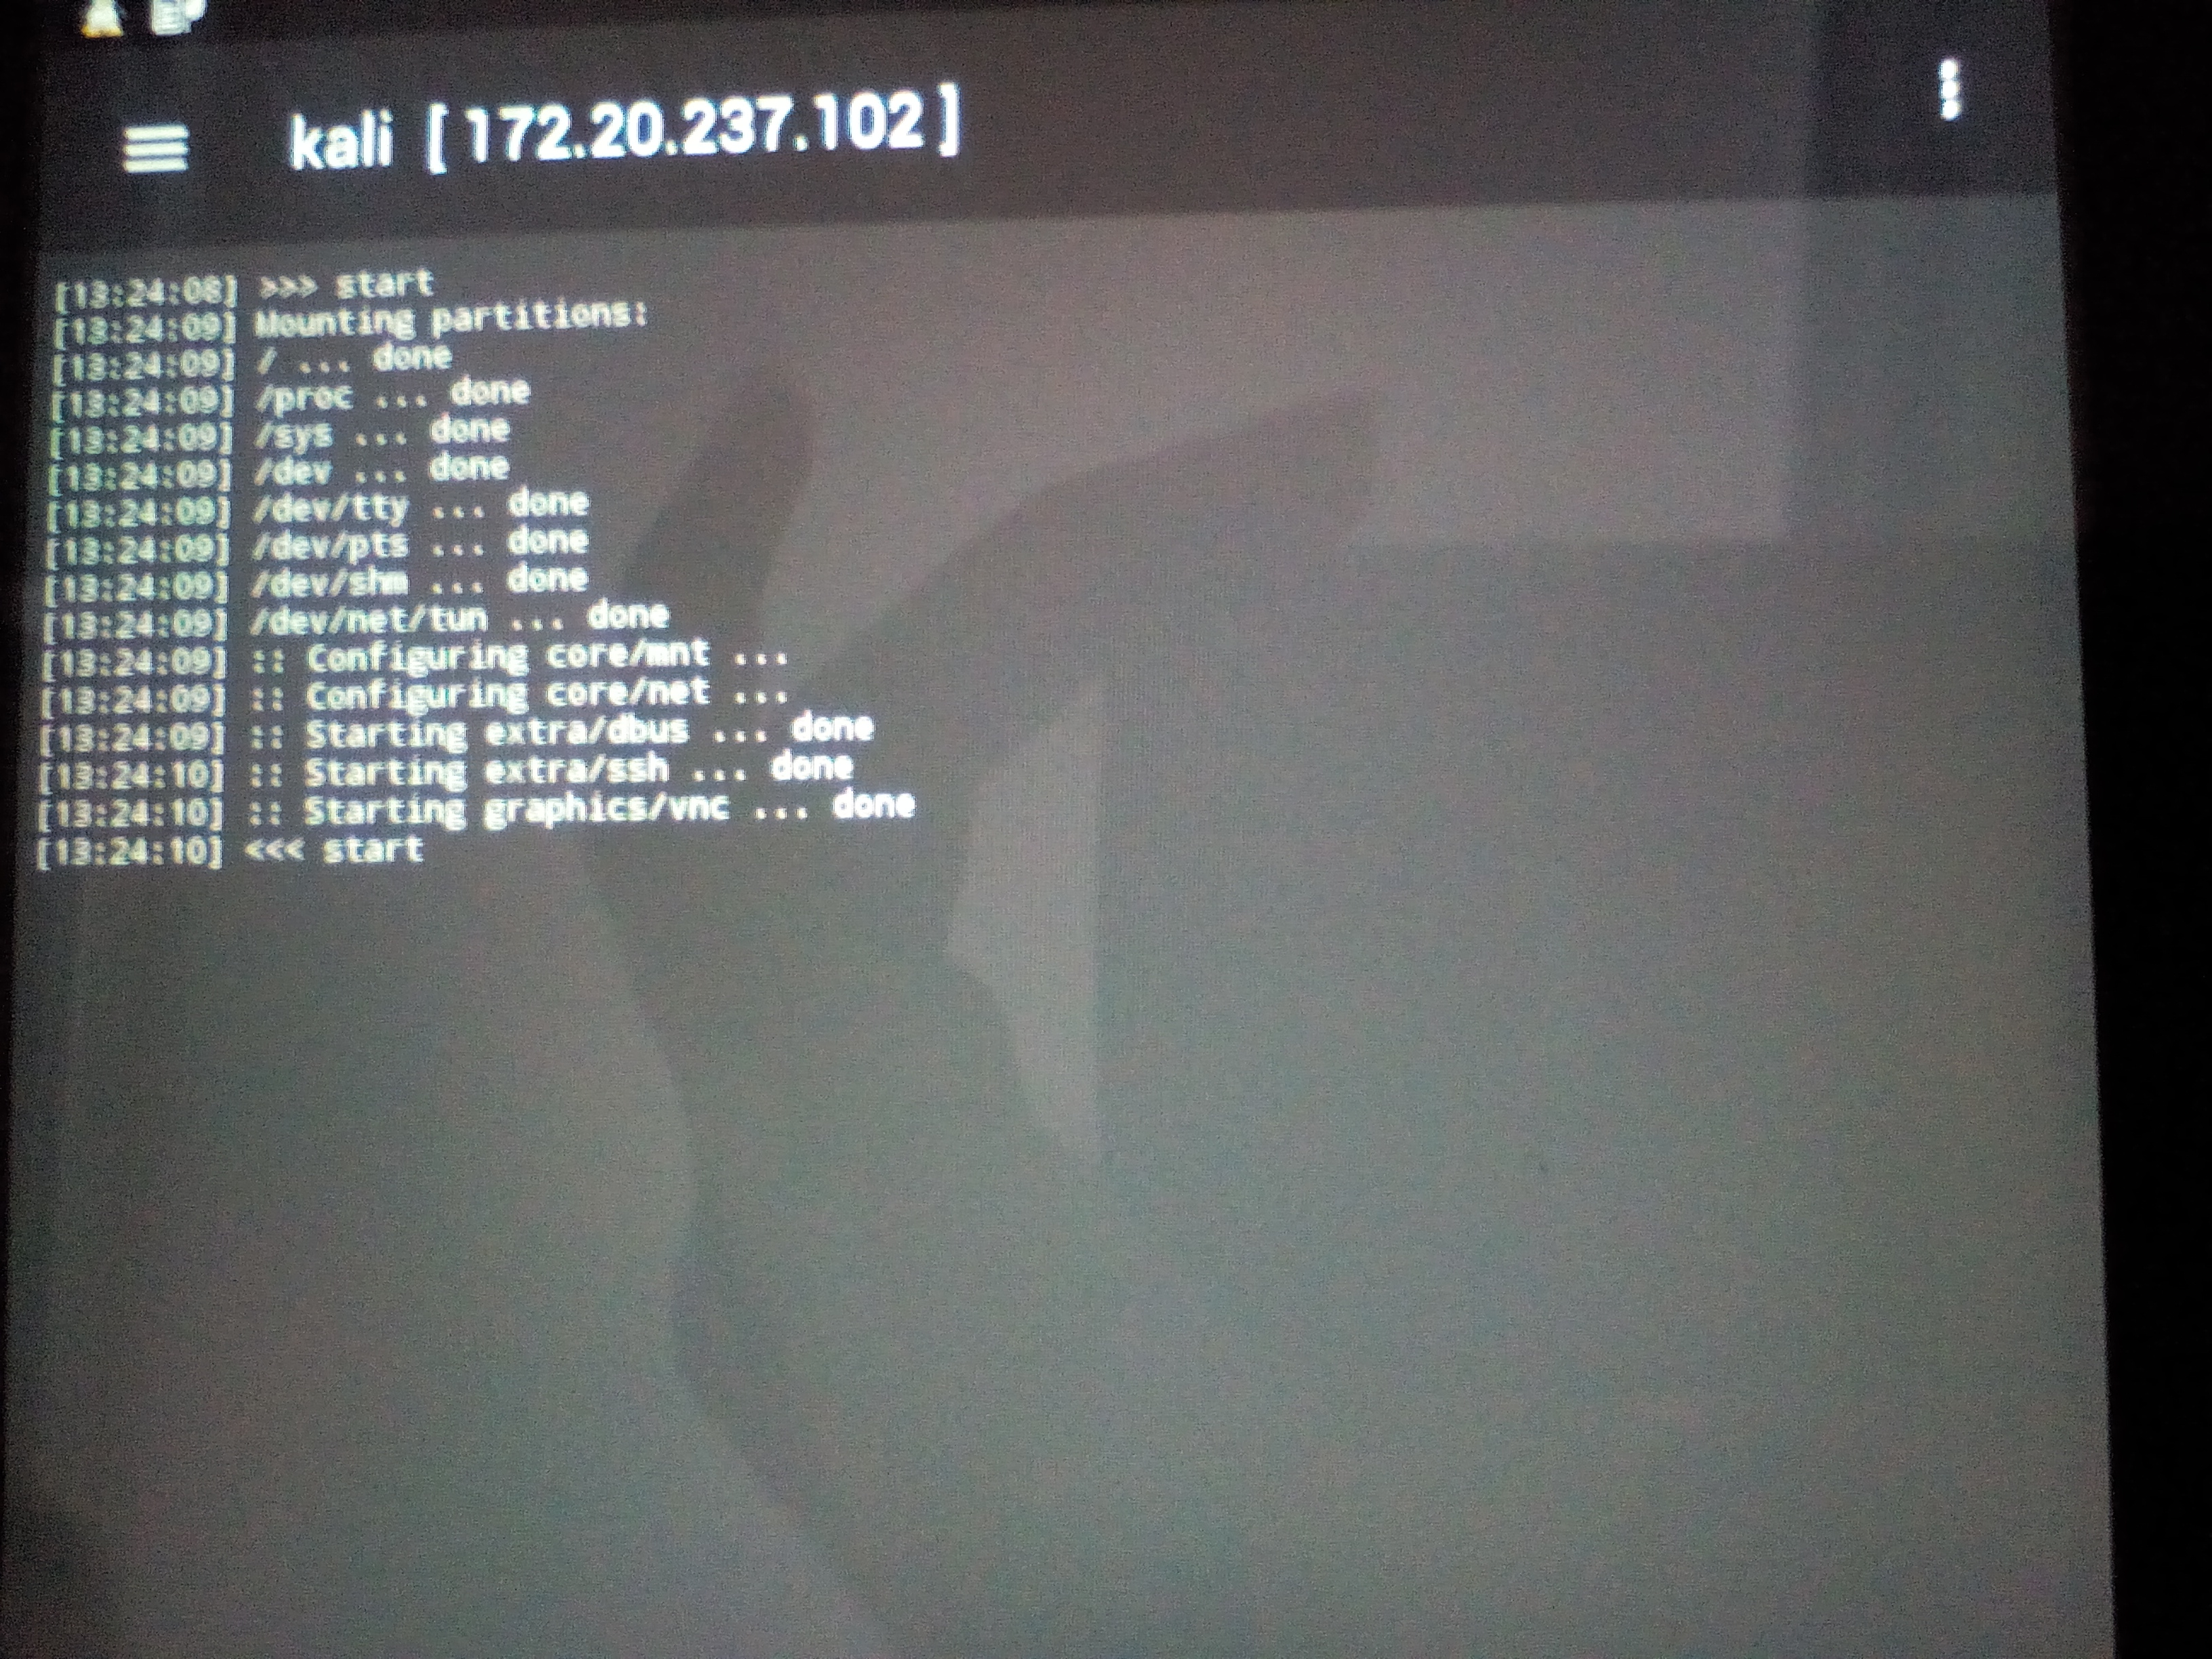
\includegraphics[scale=0.09]{./Image/img5} \\ \\
- Dann klicken auf Start \\
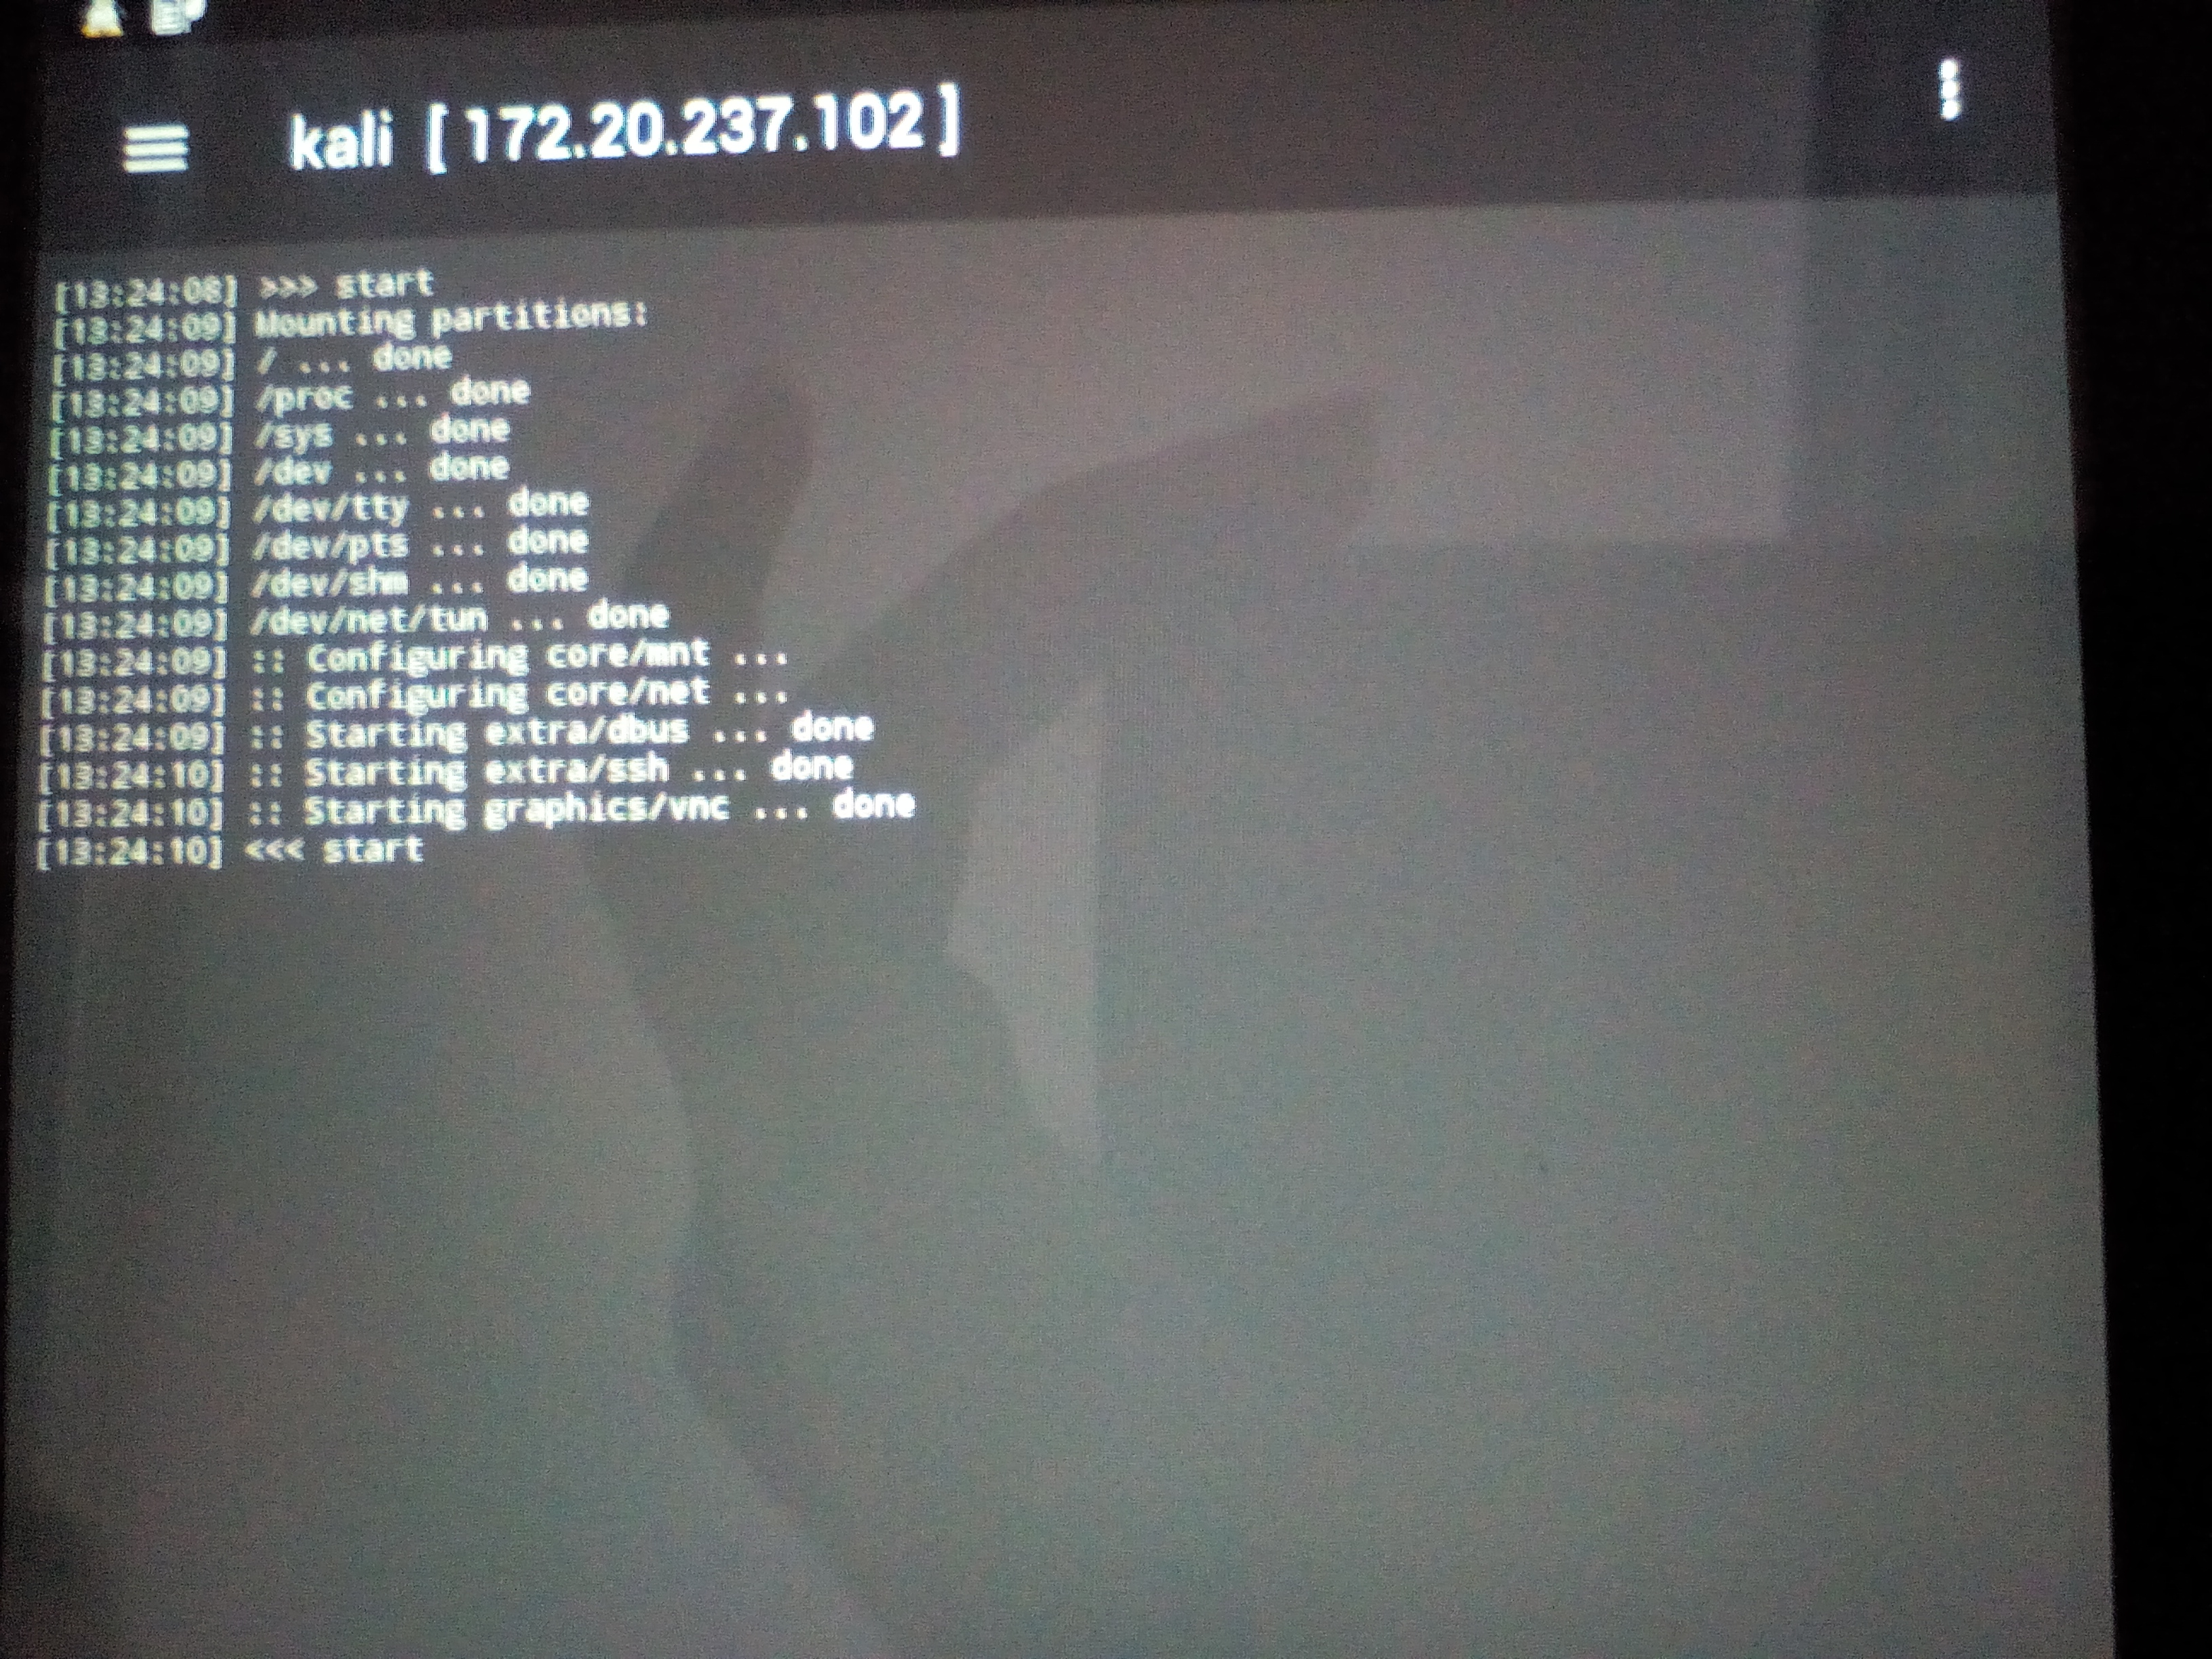
\includegraphics[scale=0.09]{./Image/img6} \\ \\
- Warten auf das Ende der Installation \\
- Klicken auf Start \\
- Sich melden an Android VNC Viewer mit der Super User Parameter \\
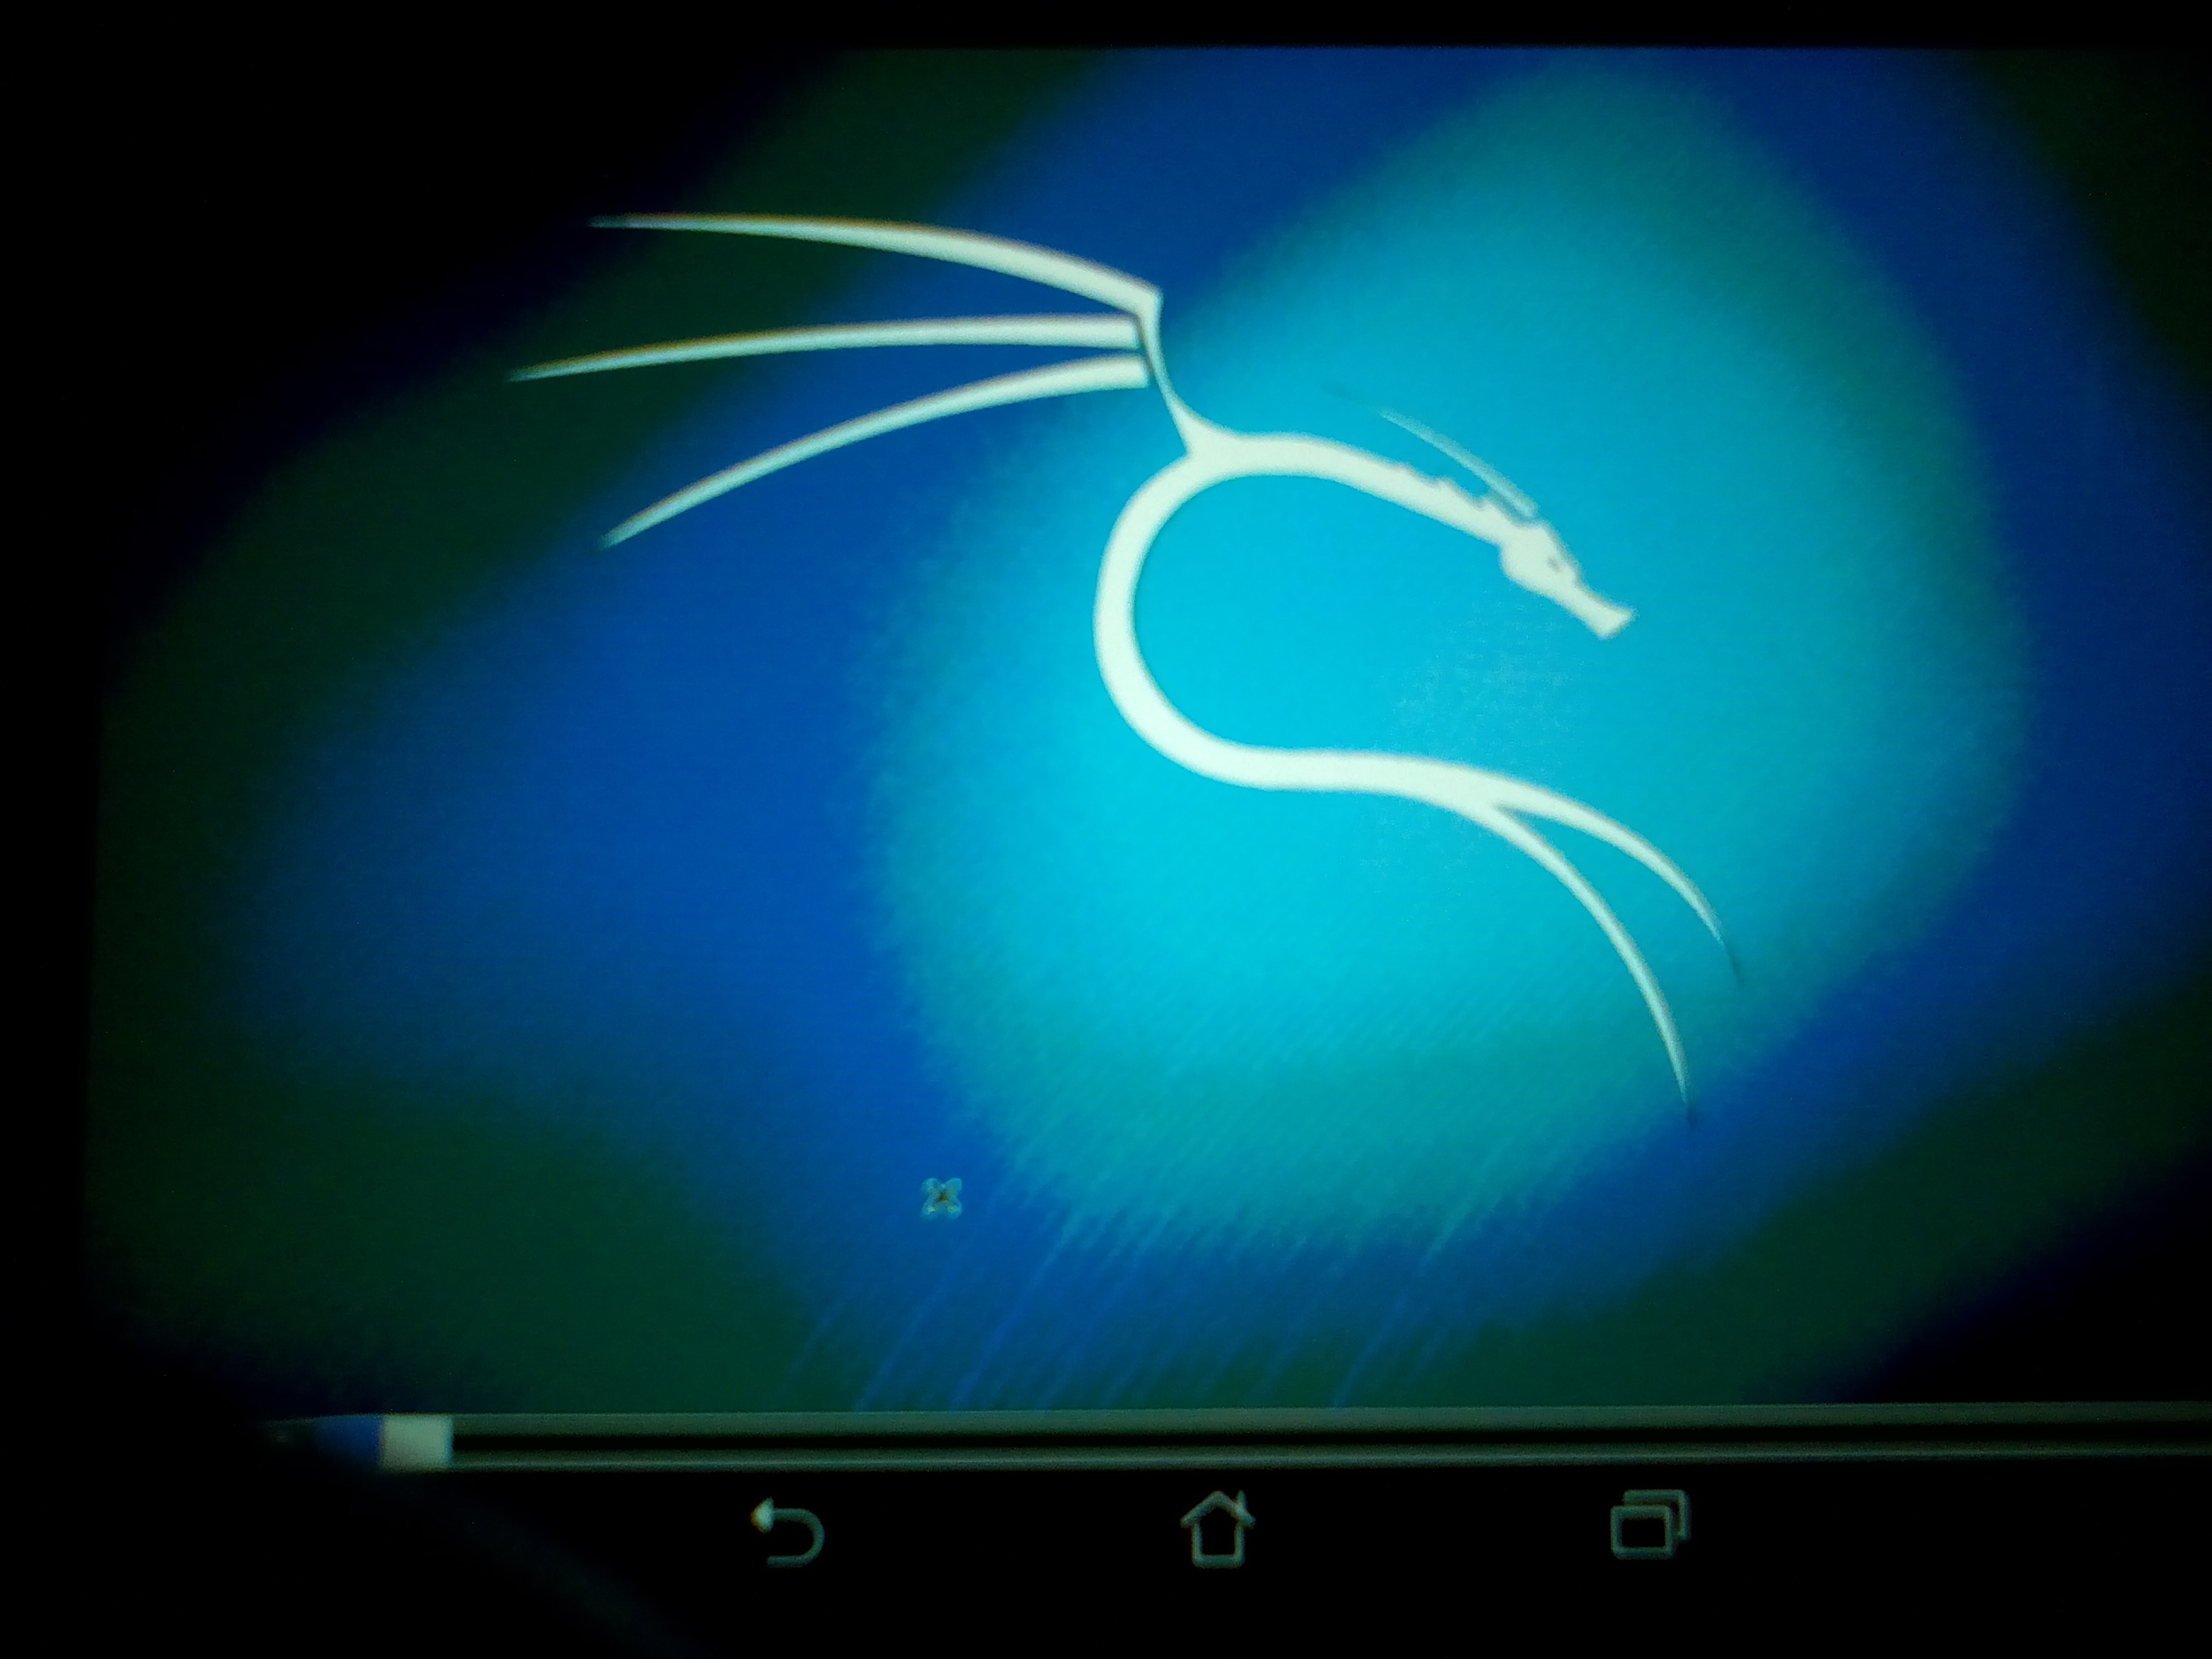
\includegraphics[scale=0.09]{./Image/img7} \\ \\
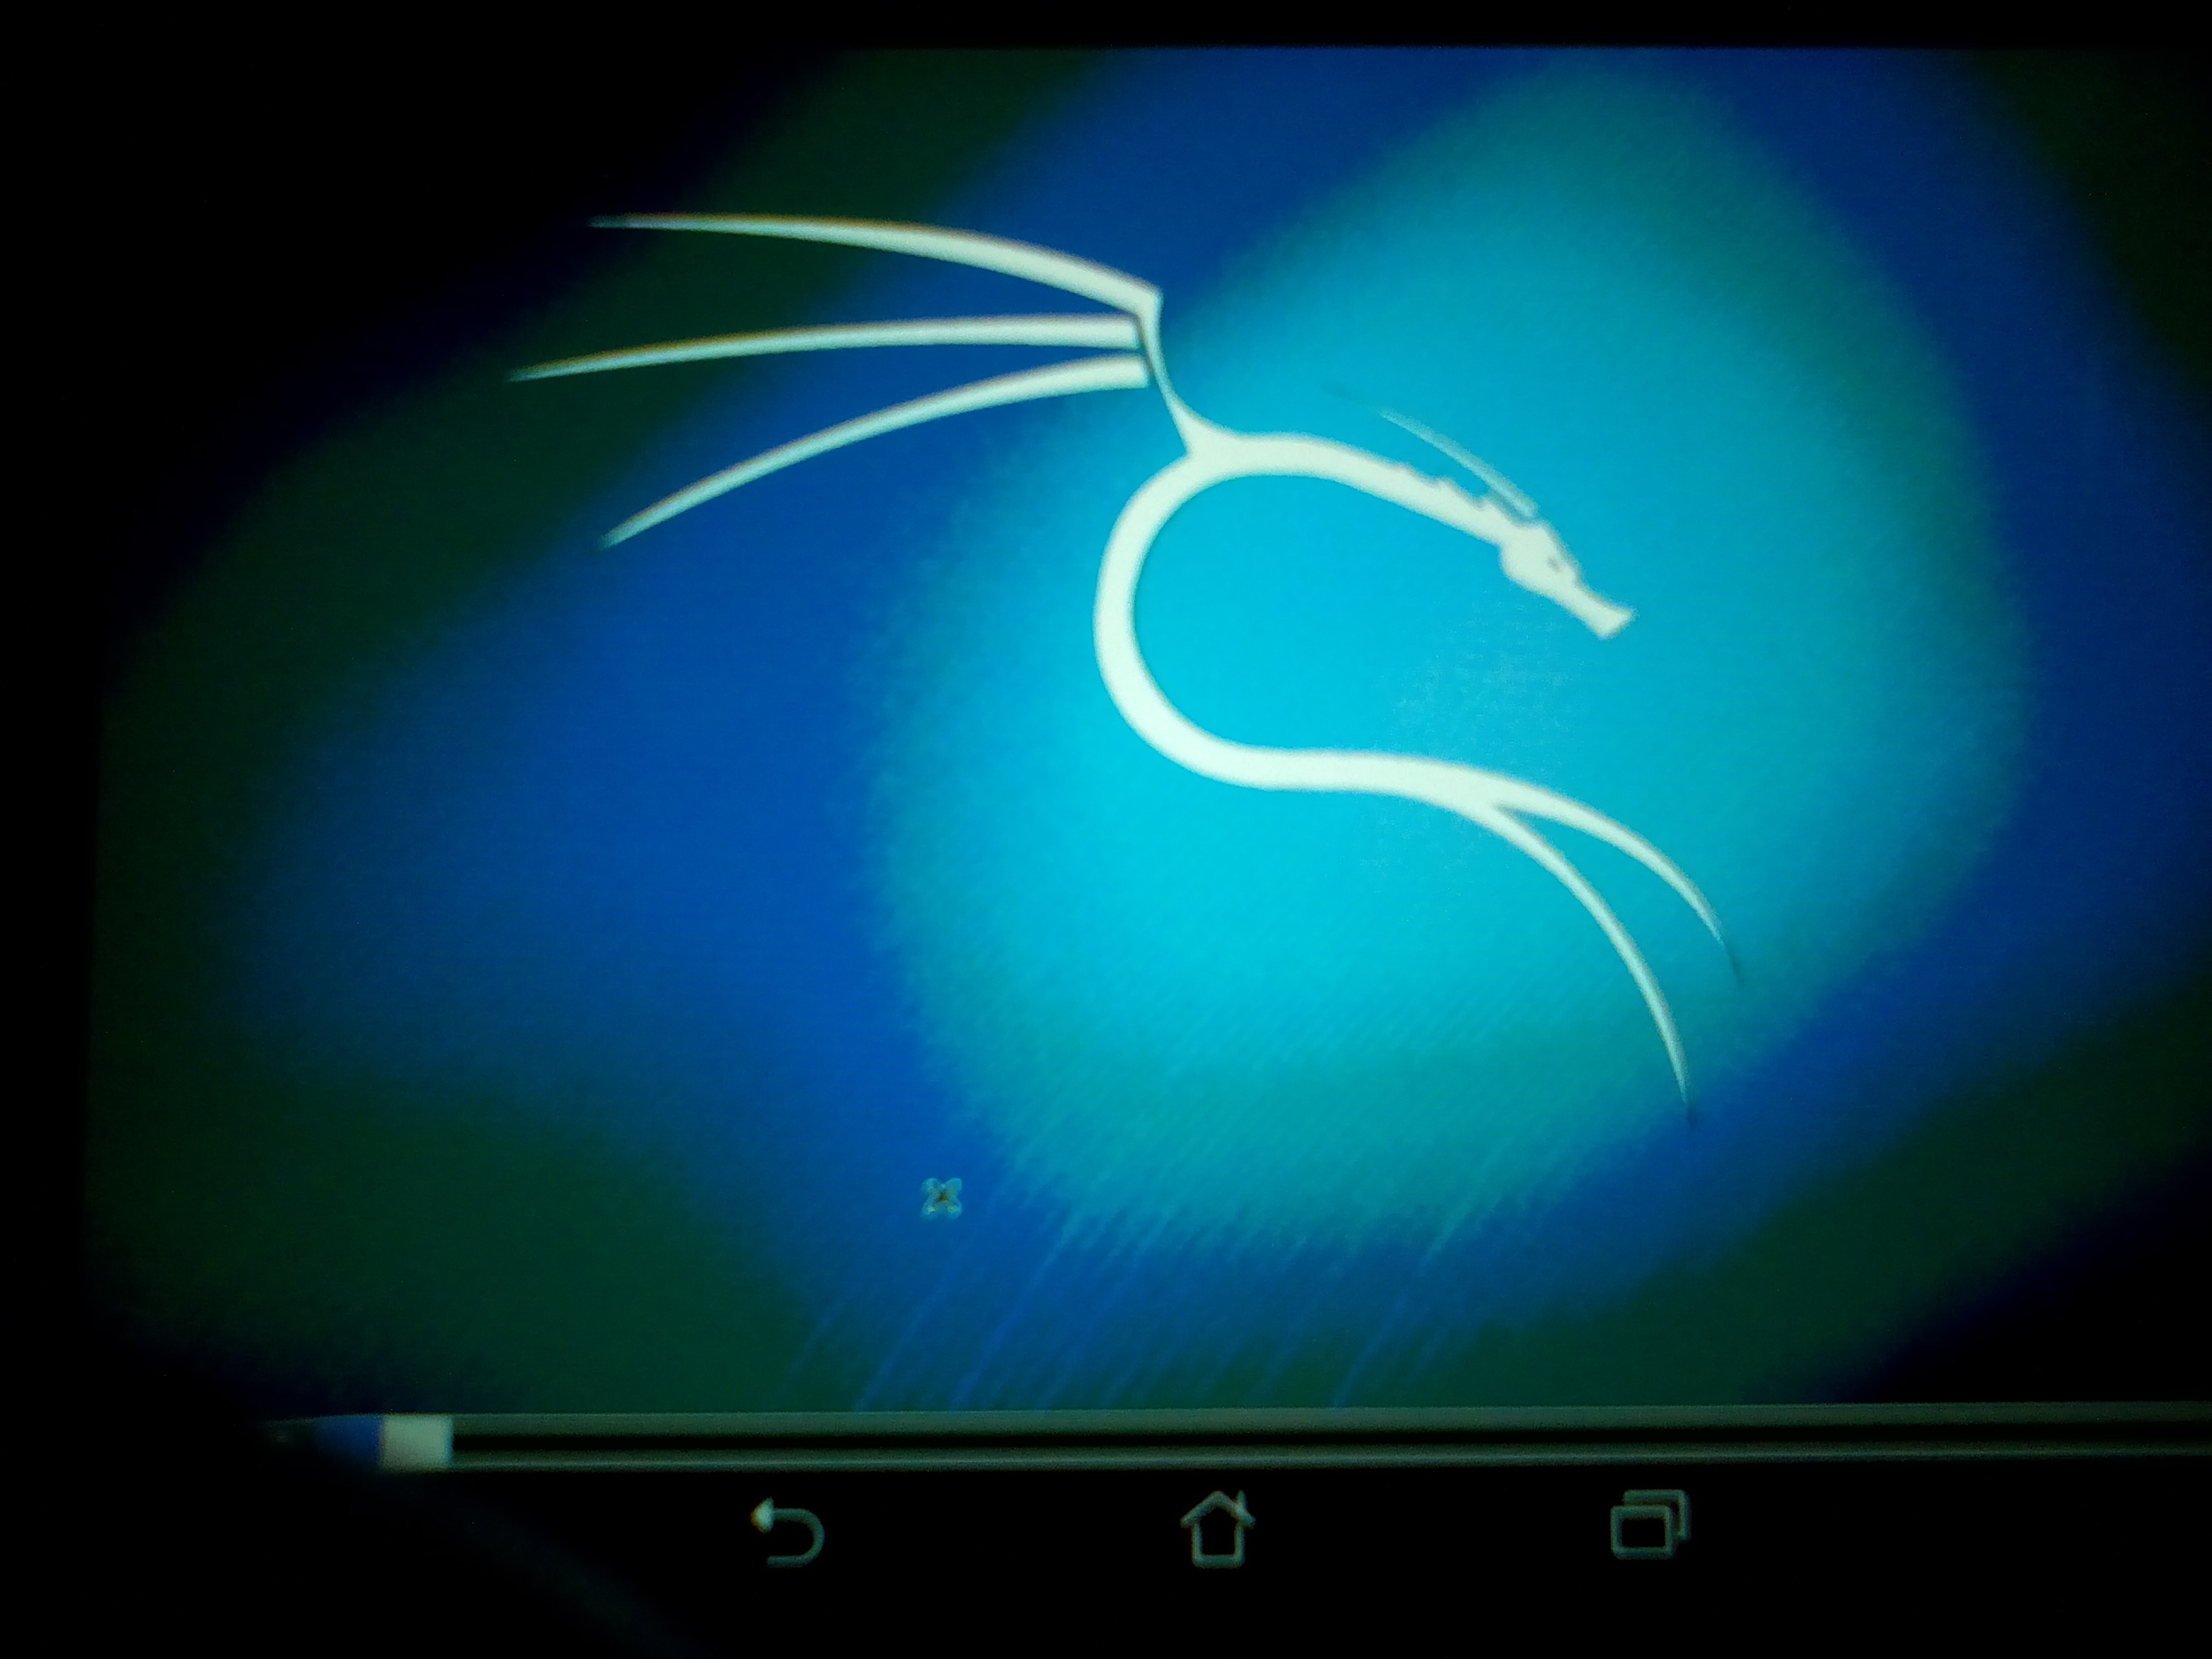
\includegraphics[scale=0.09]{./Image/img8} \\ \\

Literatur: http://www.compsmag.com/install-kali-linux-android/

\section {Installation von Nethunter auf Nexus Geräte}

- Backup machen vor der Installation \\  
- Das Gerät muss gerootet sein \\
- Wir erhalten die Administrator-Rechte durch Super-SU \\
- Vorraussetzung: Laden die richtige Version von Nethunter für Nexus 7 Android 5.1.1 herunter (Lilopop) \\
- Die Installation erfolgt durch TWRP Manager \\ 
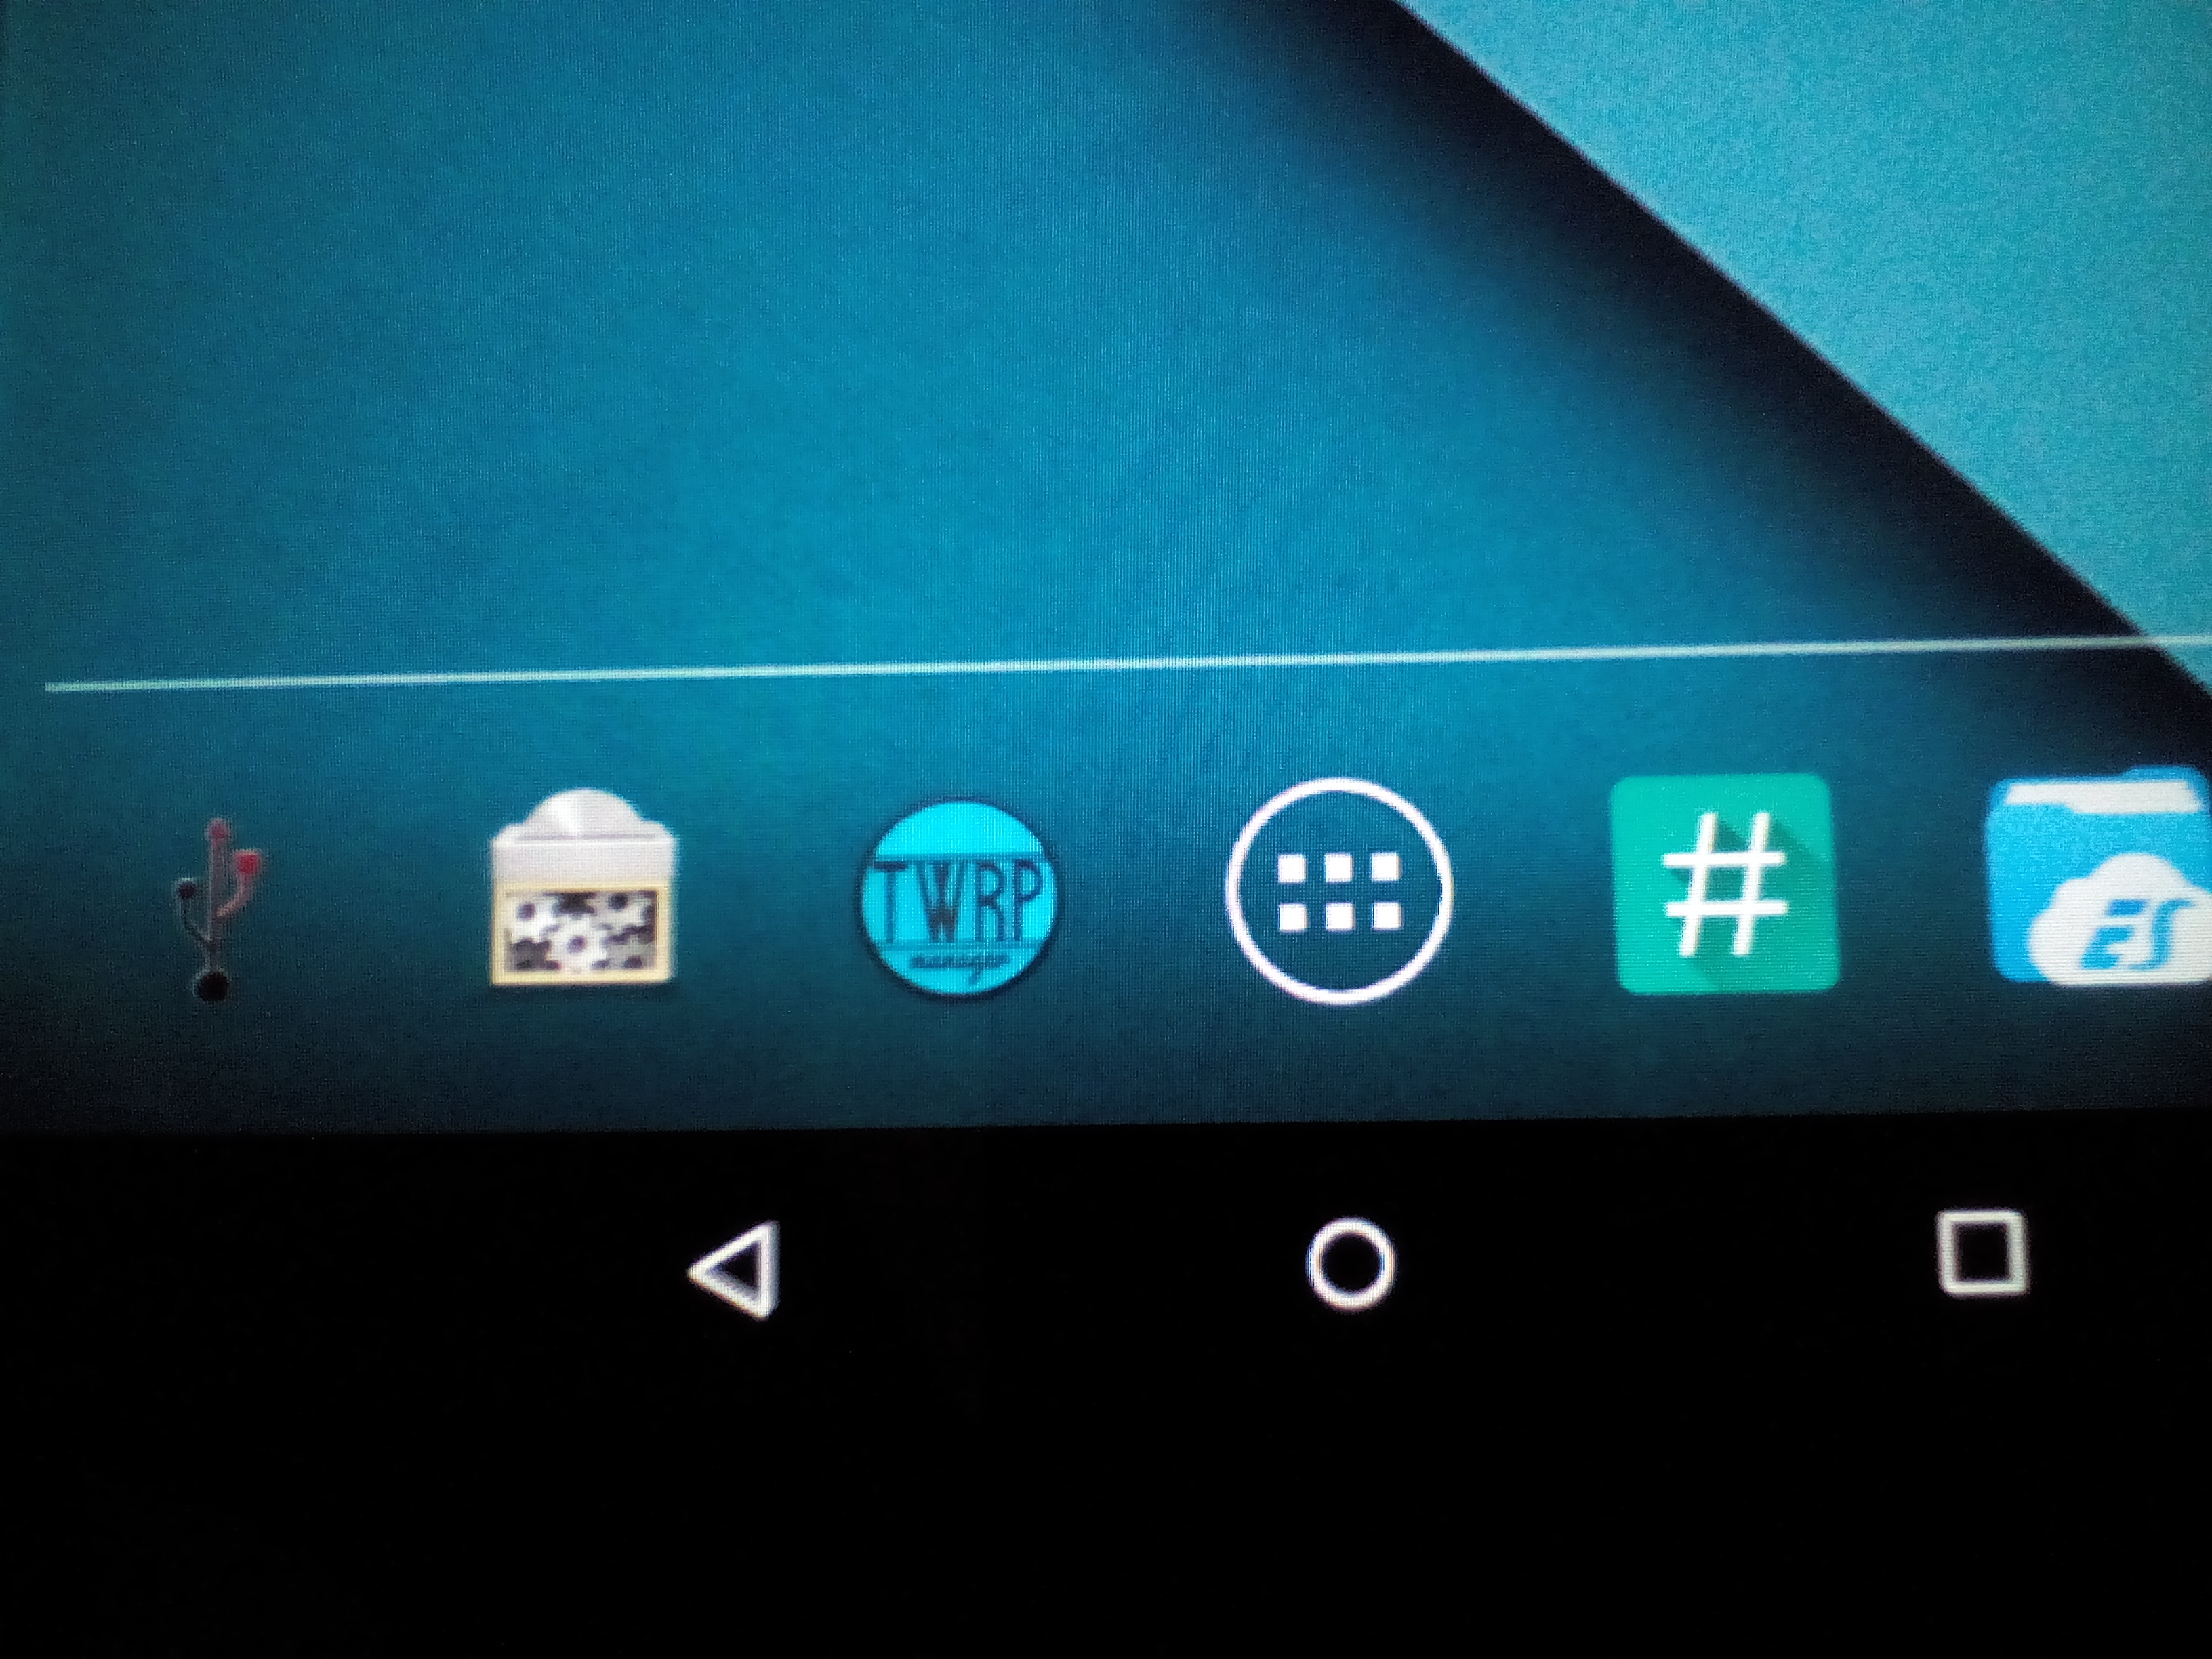
\includegraphics[scale=0.09]{./Image/img9} \\ \\ 
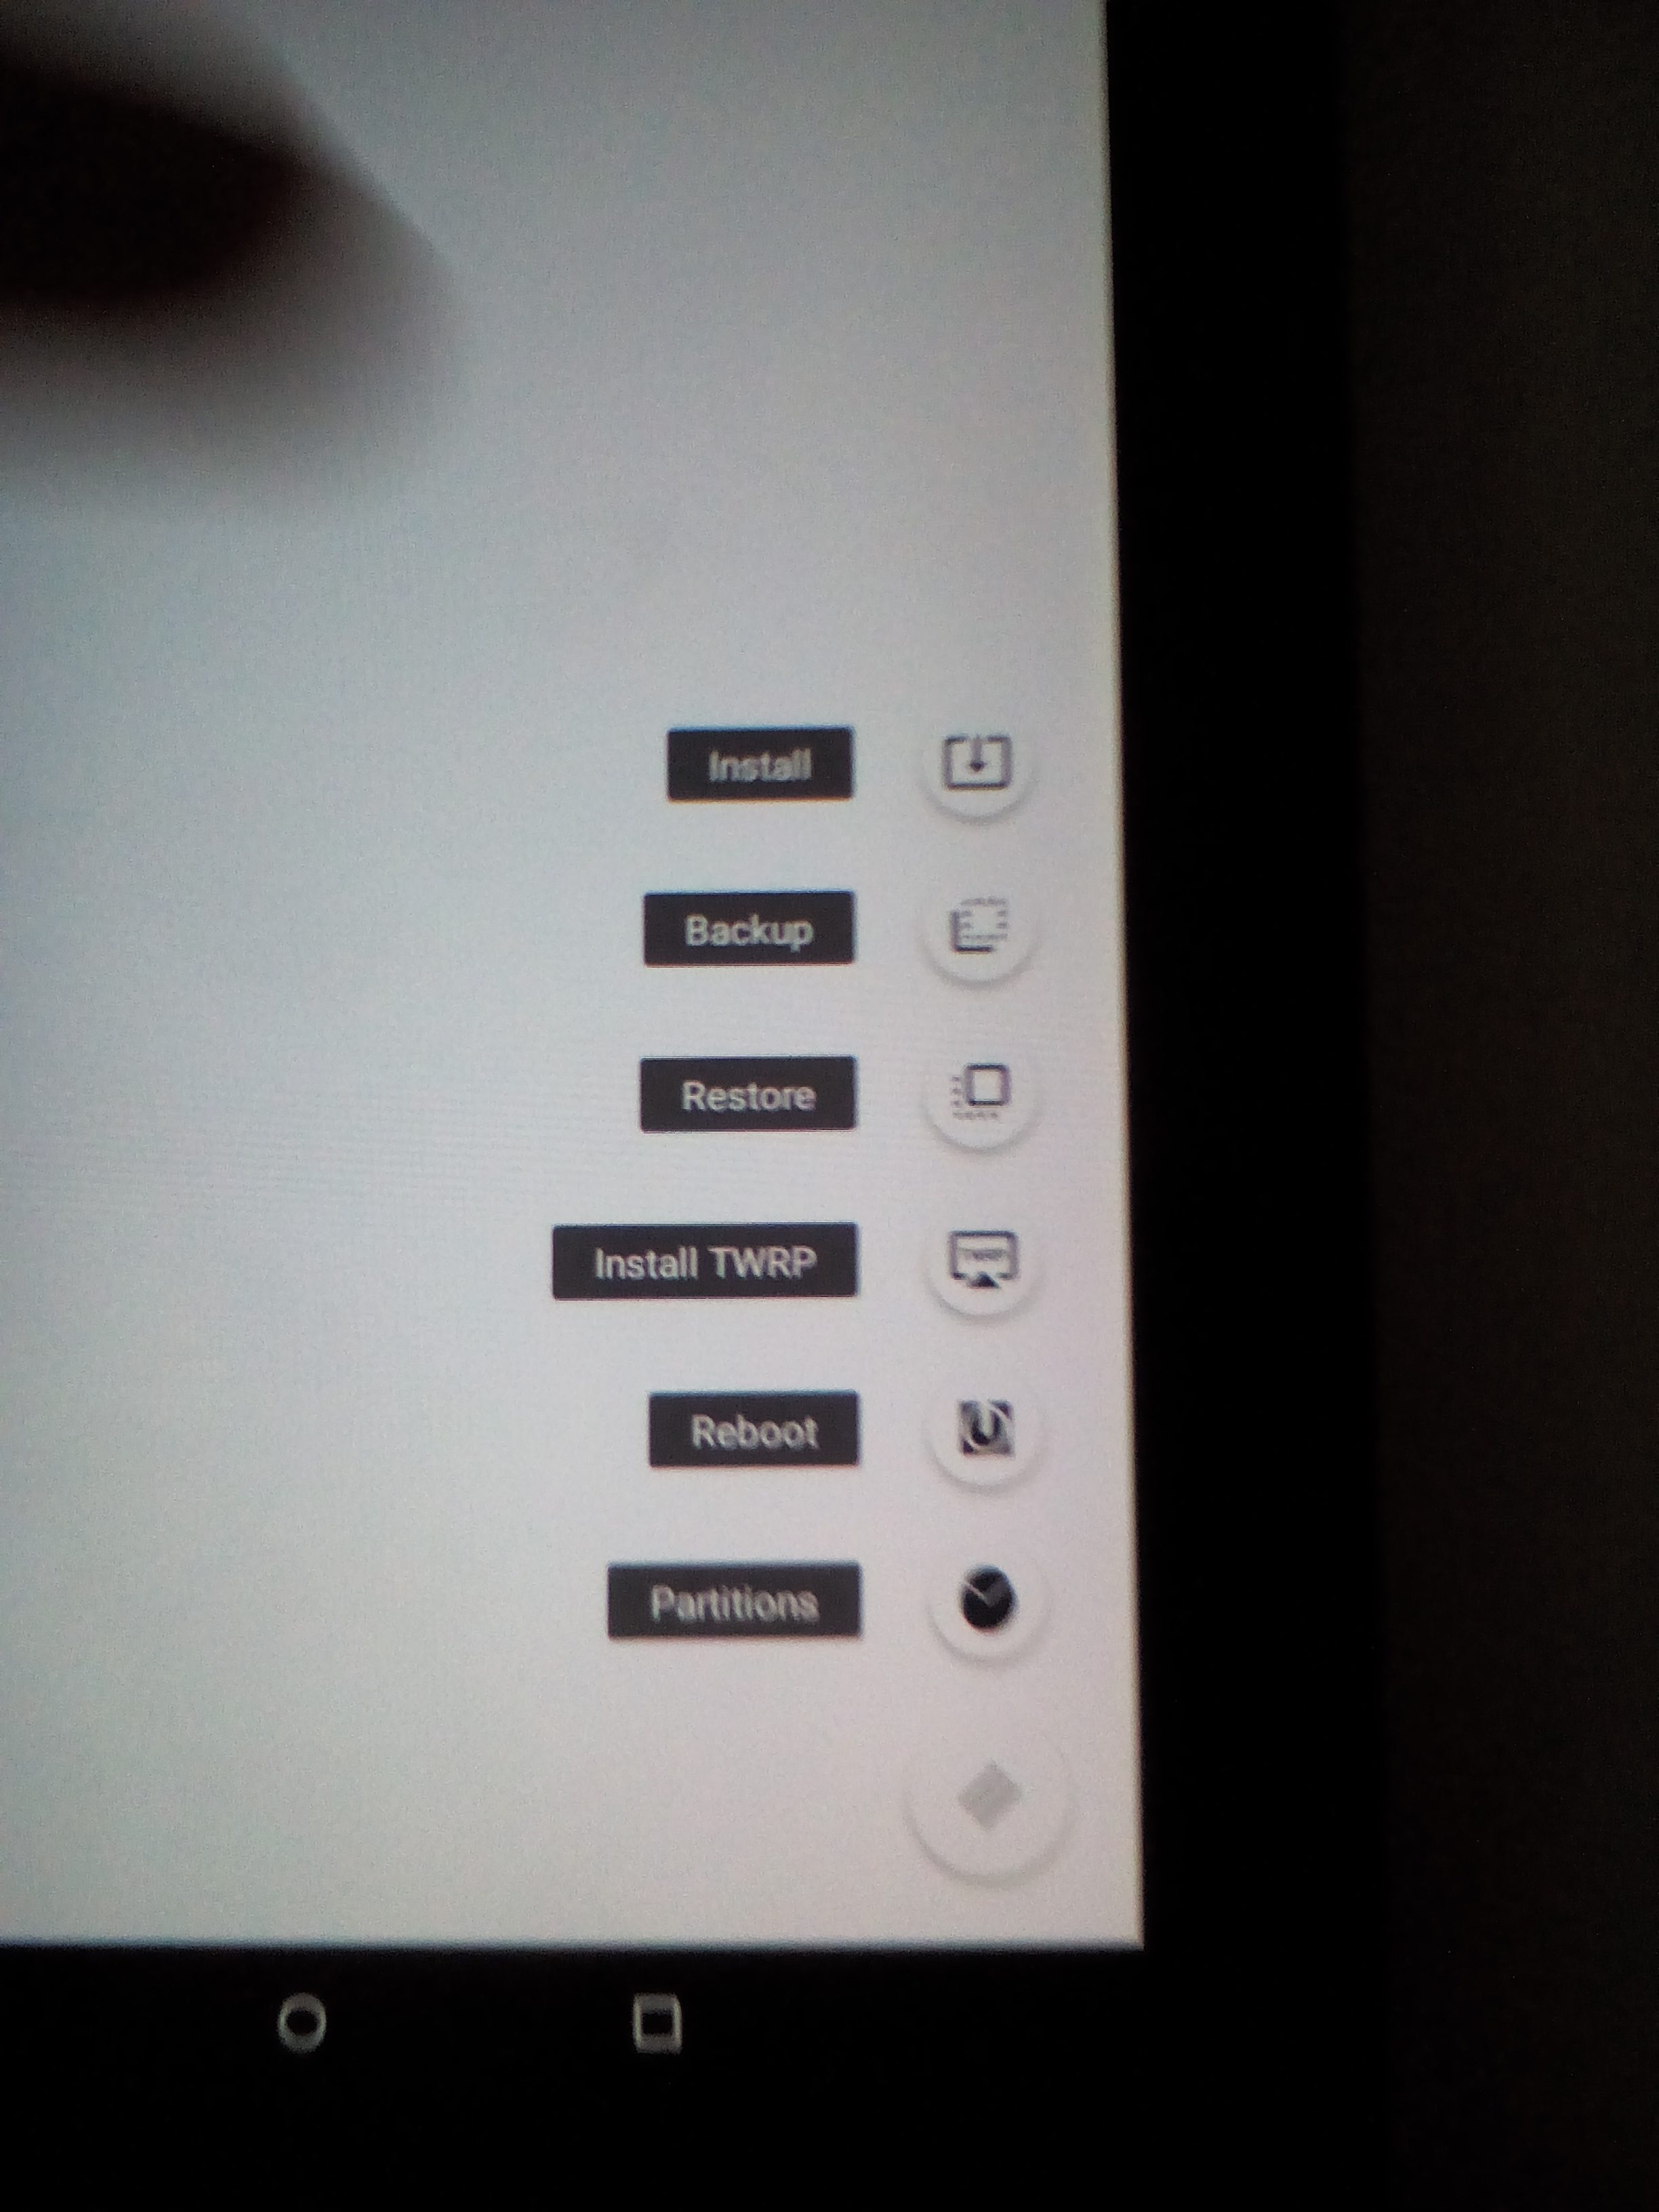
\includegraphics[scale=0.09]{./Image/img10} \\ \\
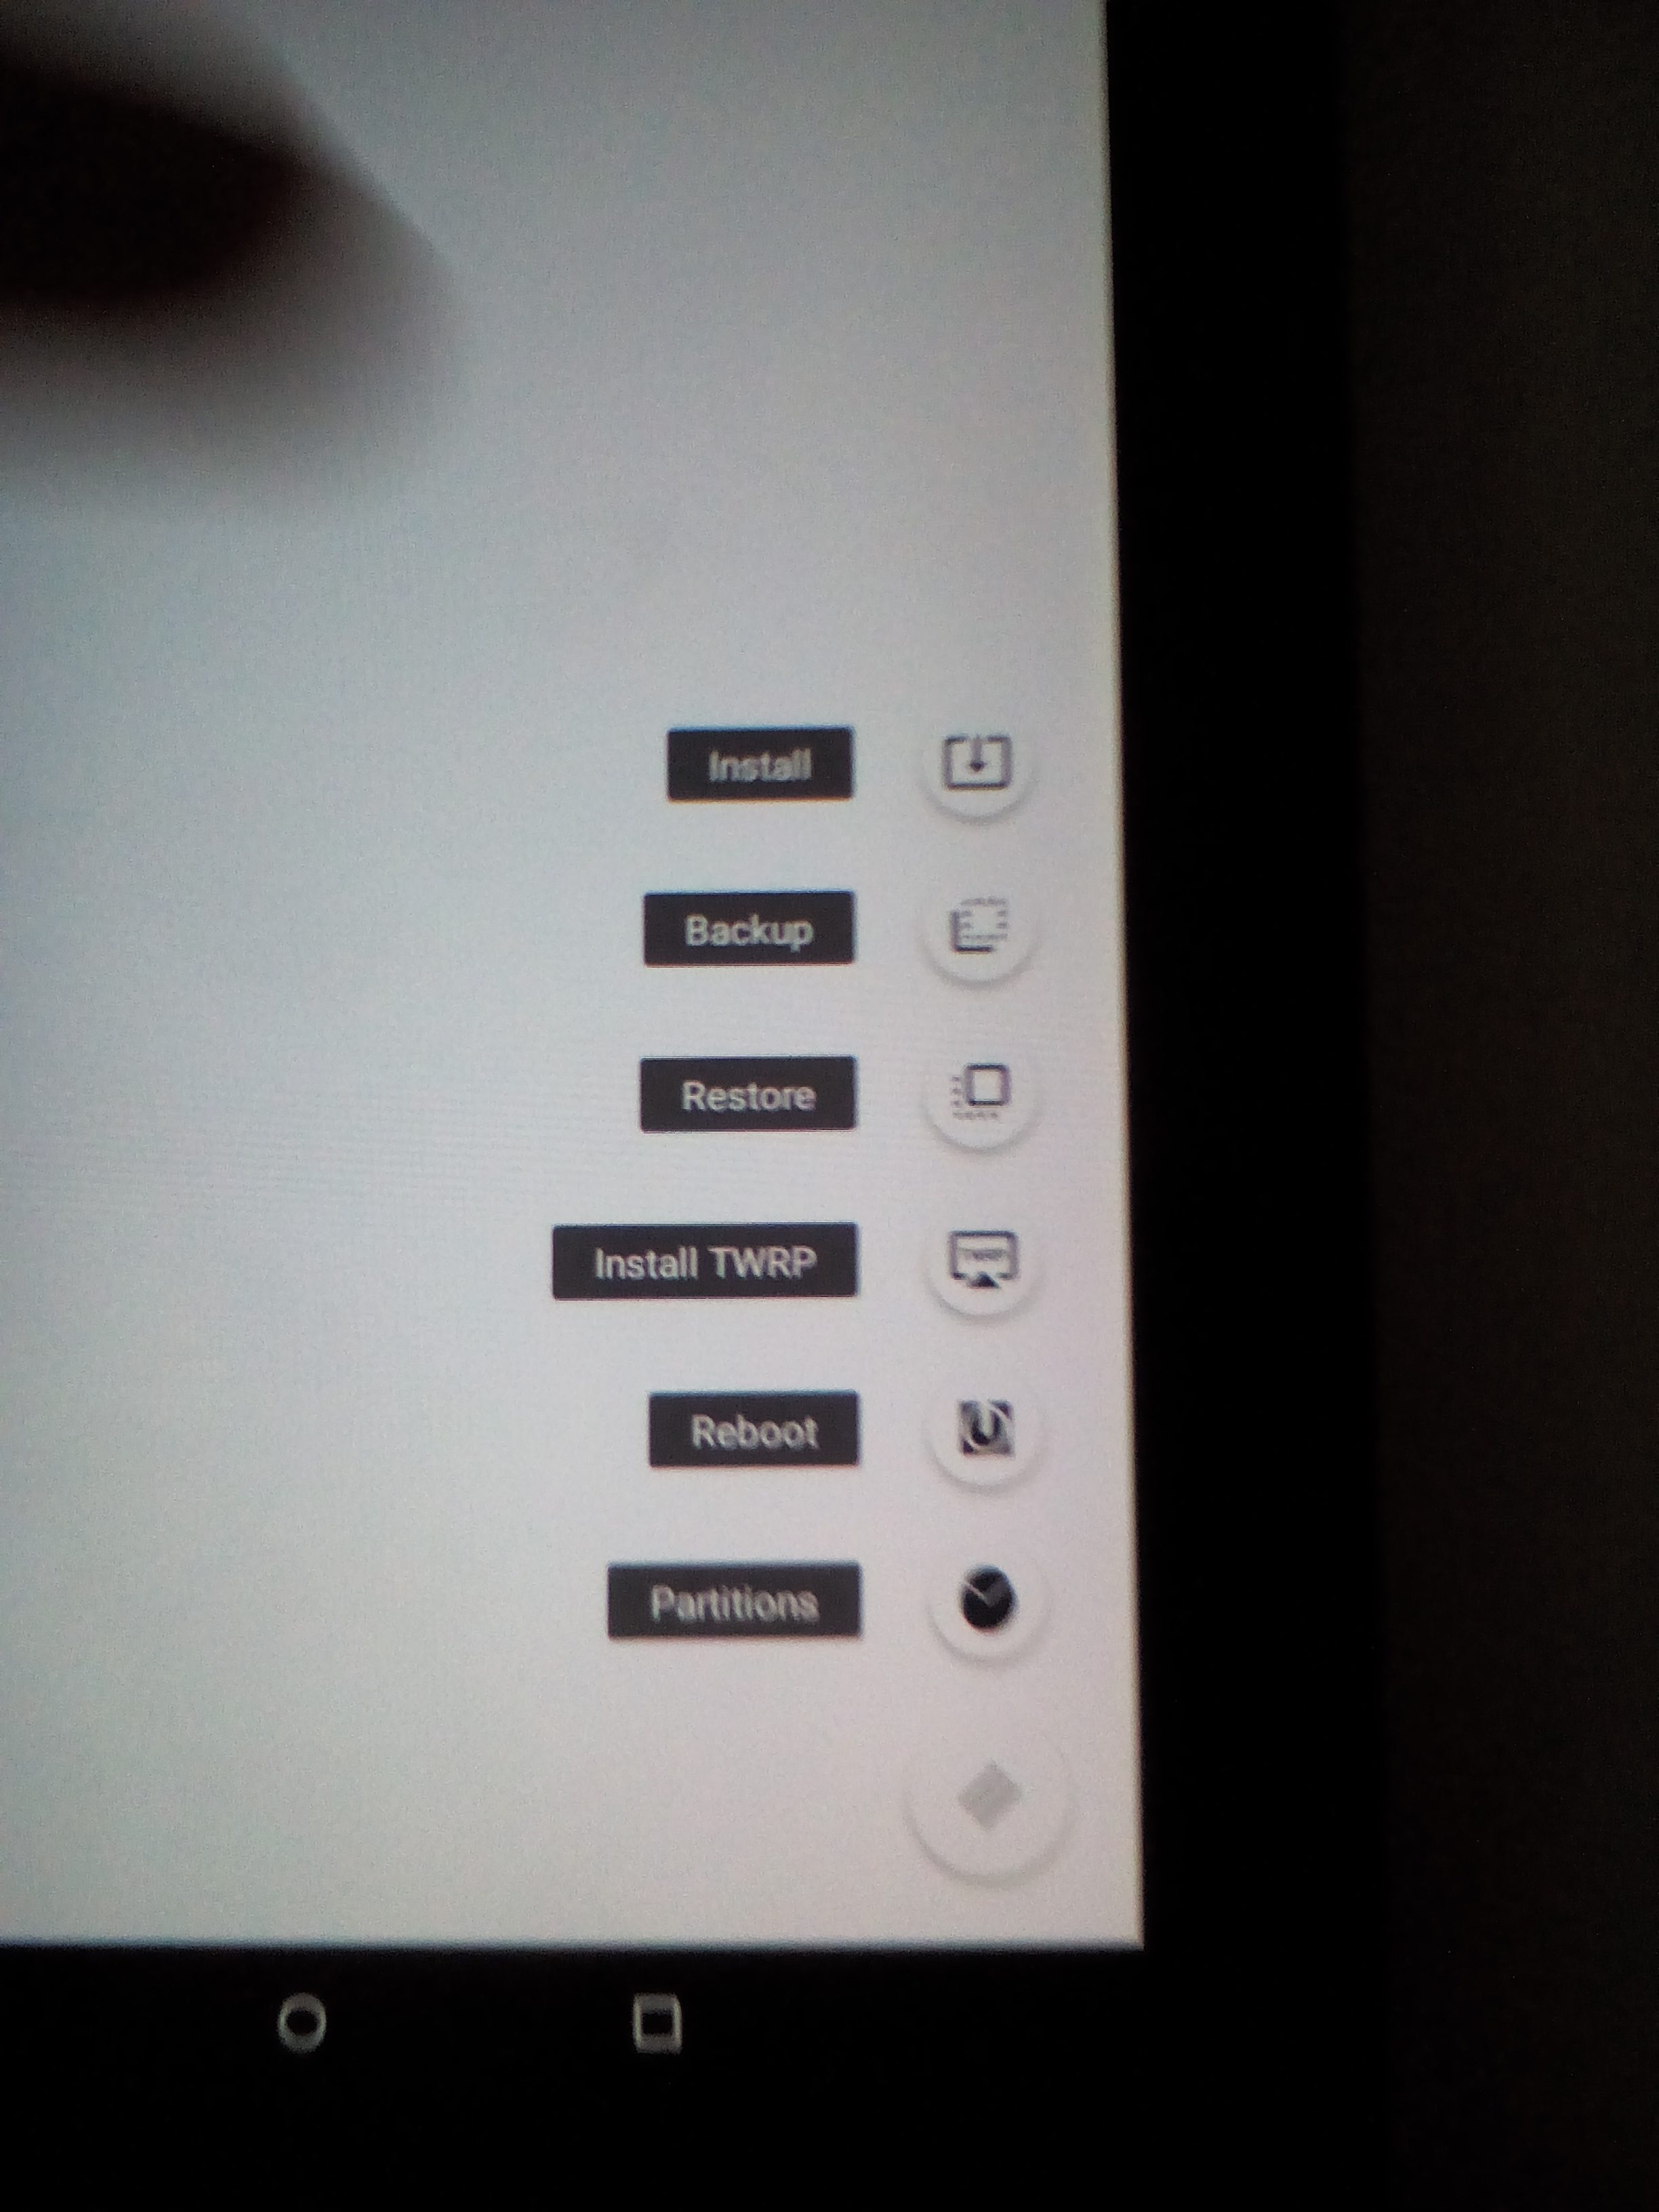
\includegraphics[scale=0.09]{./Image/img11} \\ \\ \\
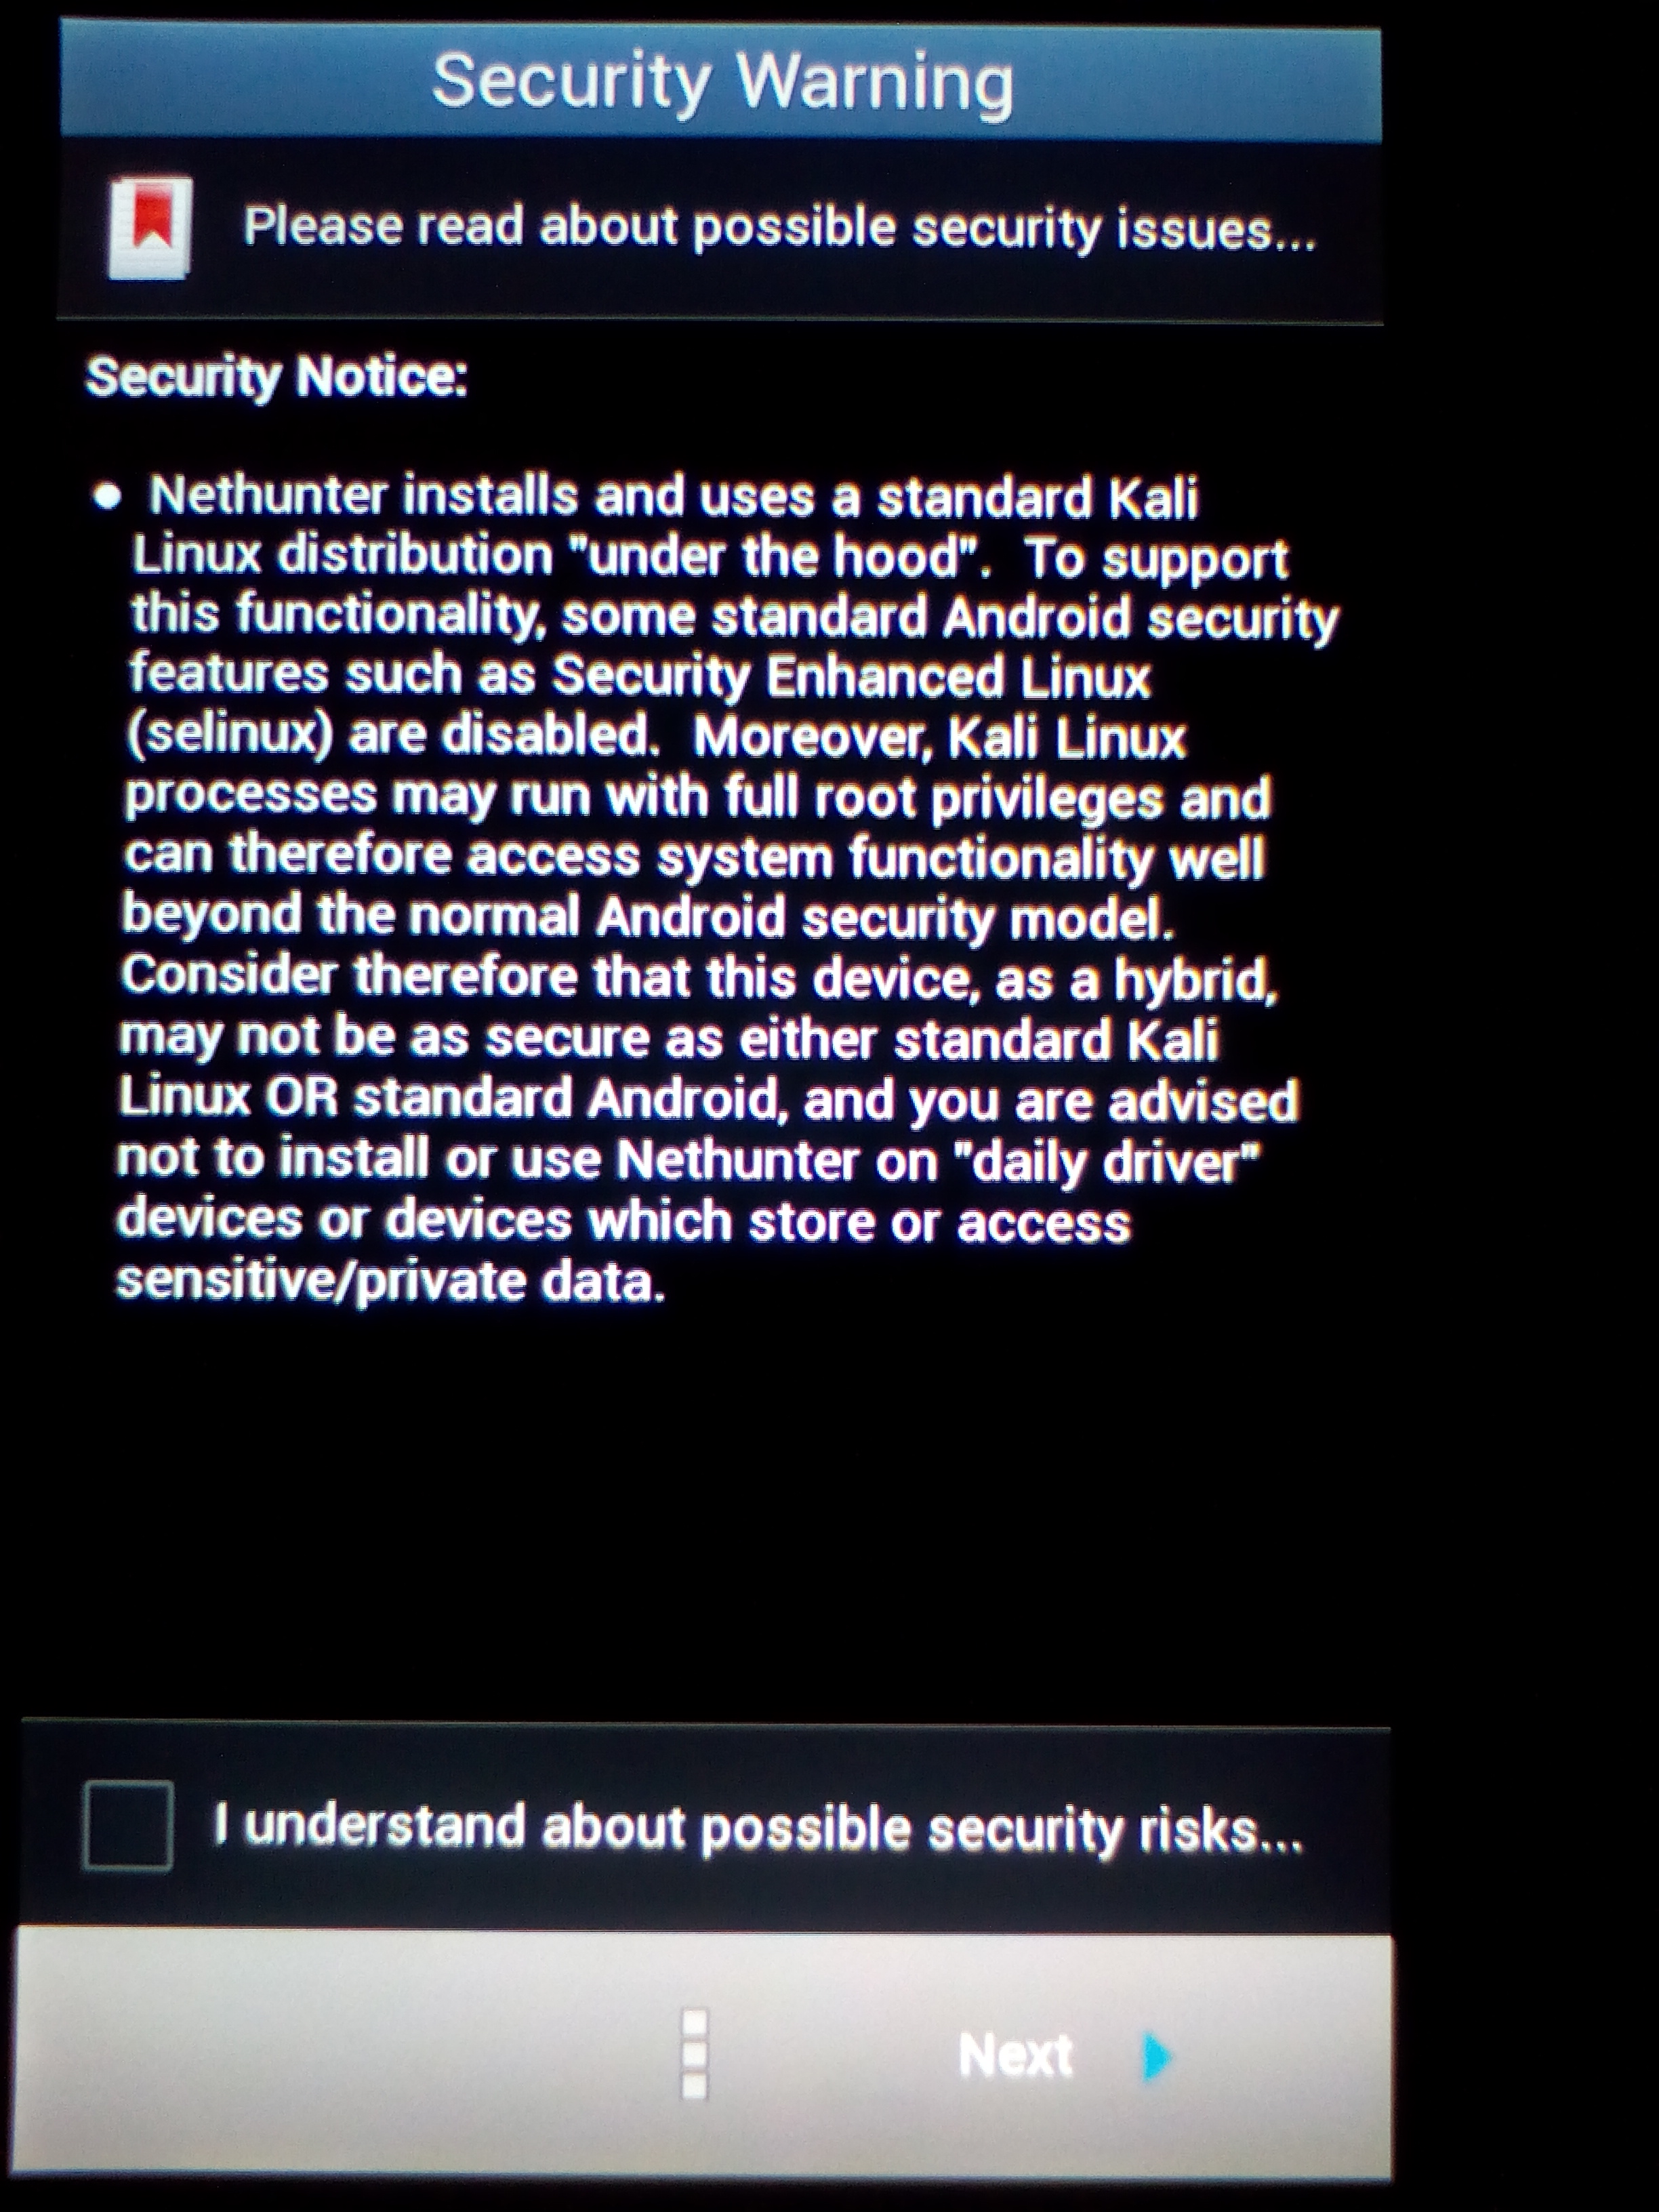
\includegraphics[scale=0.09]{./Image/img12} \\ \\ \\
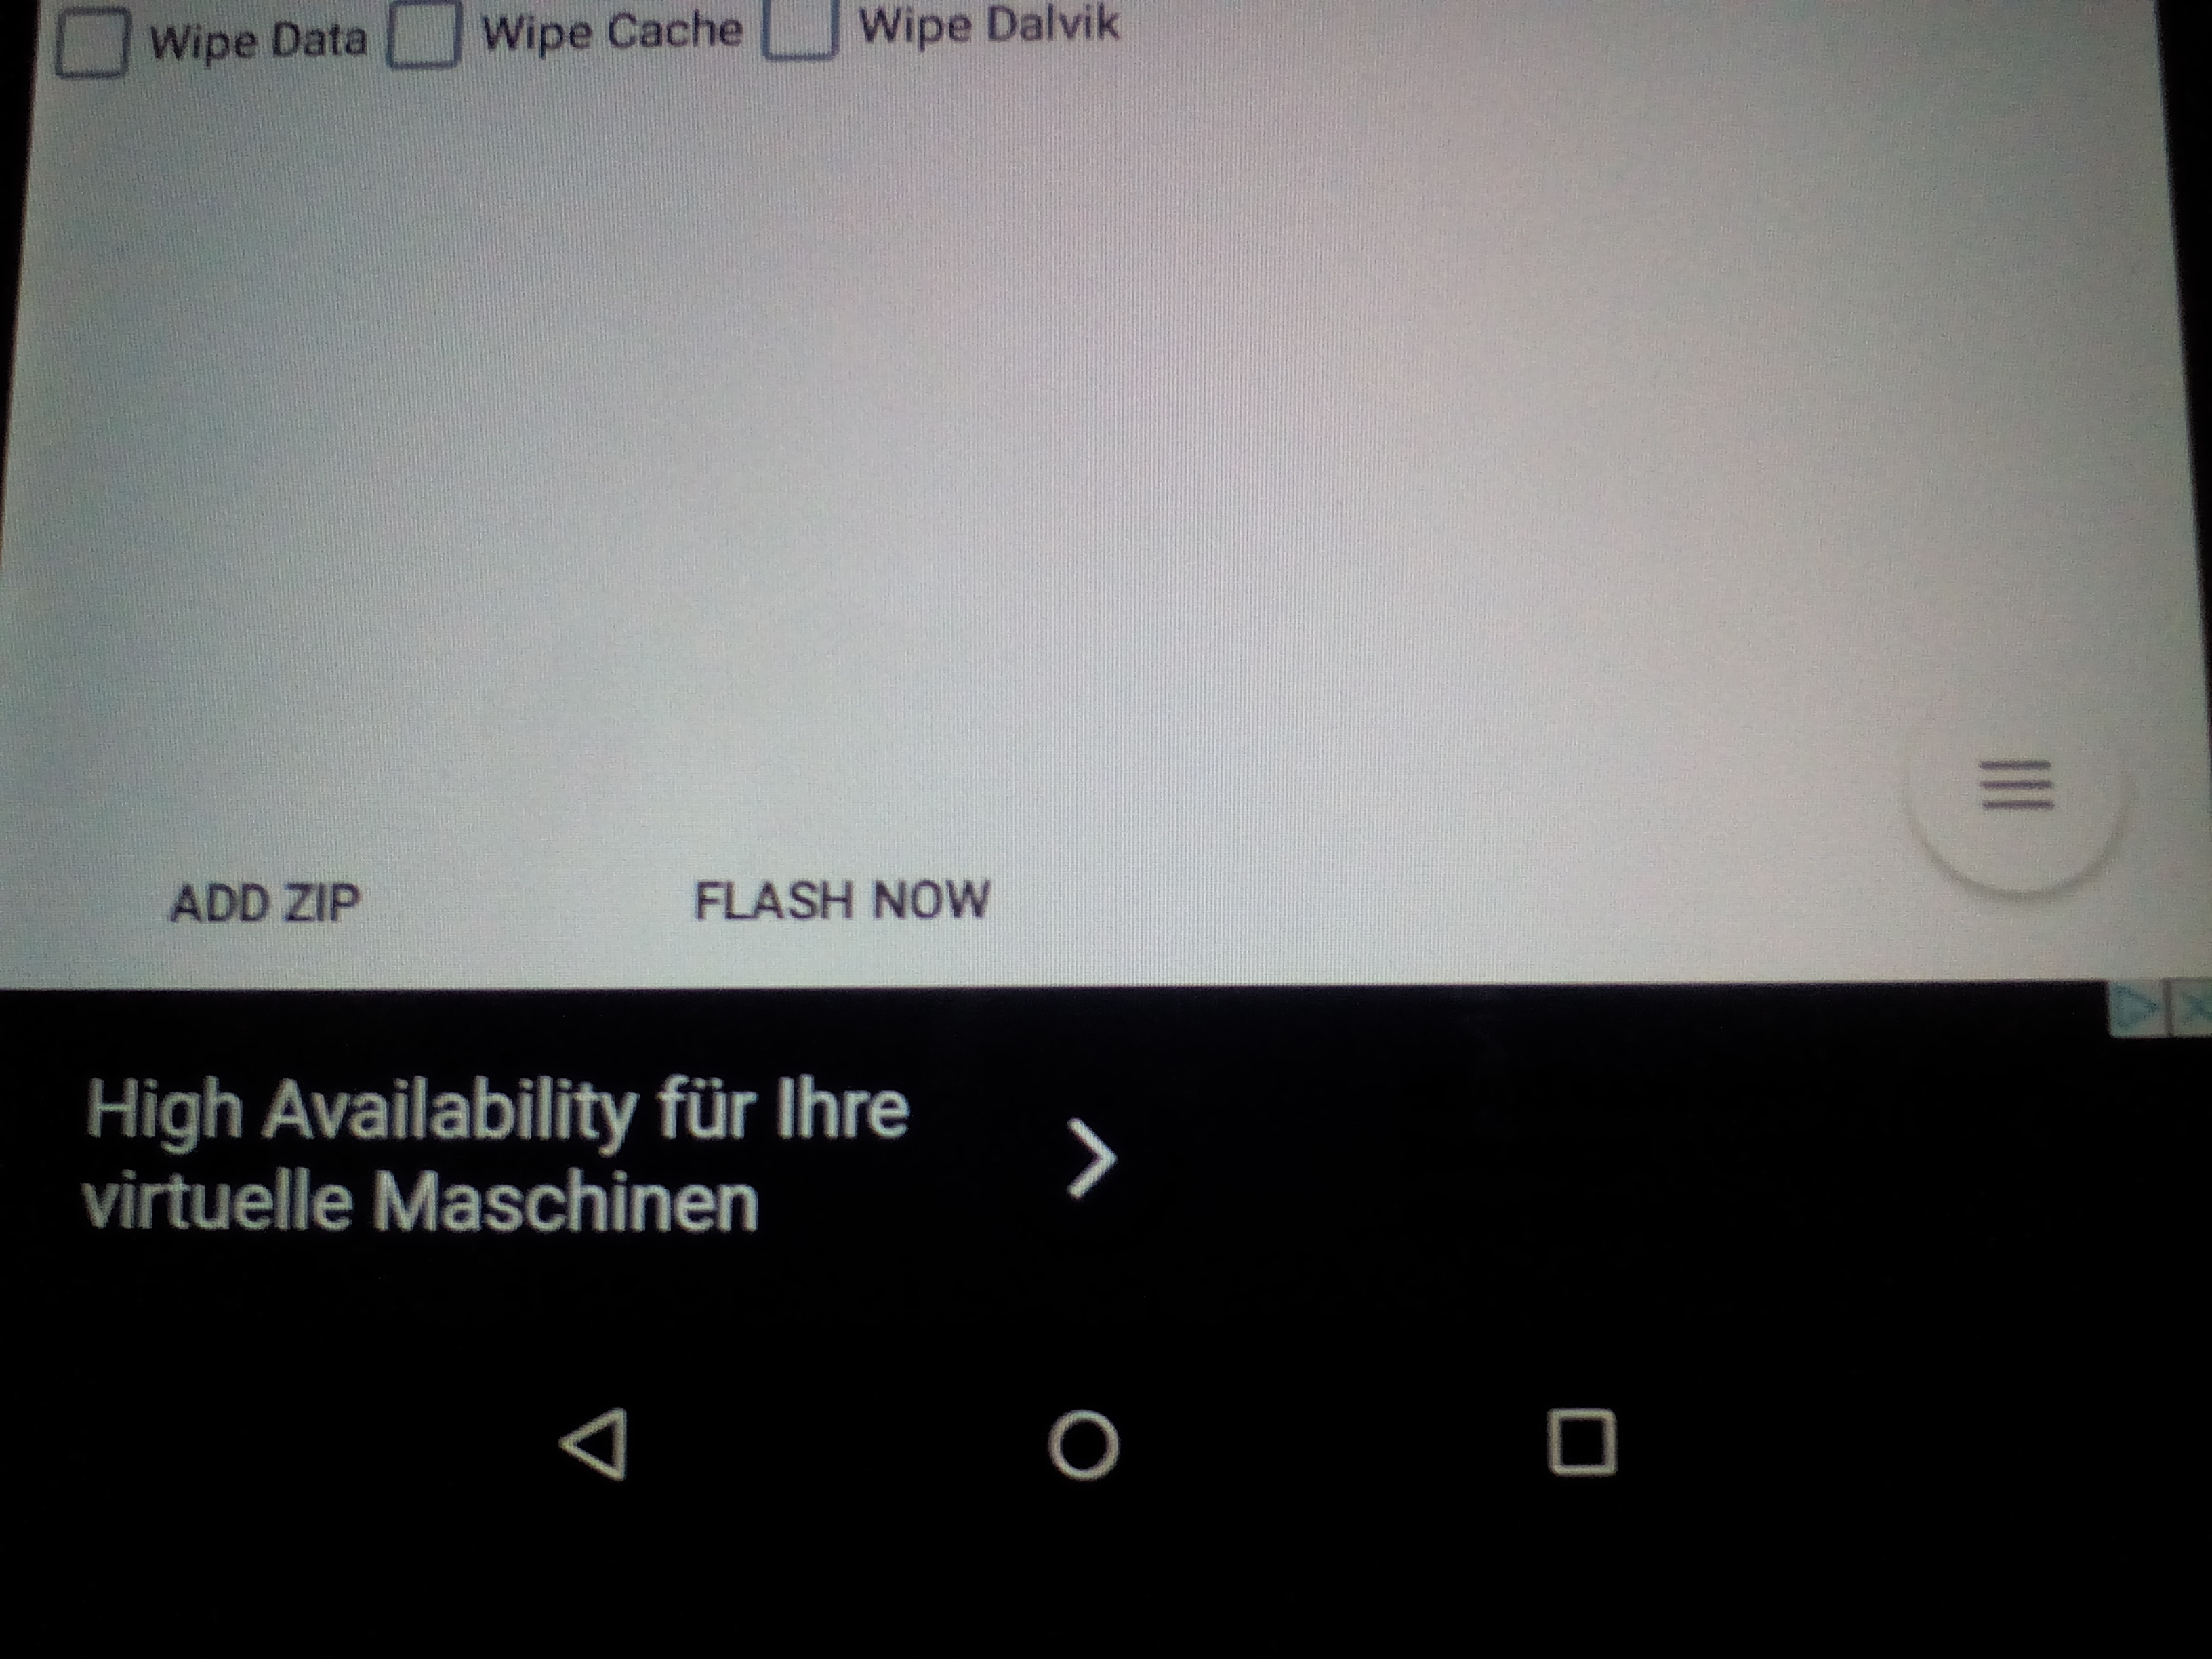
\includegraphics[scale=0.09]{./Image/img13} \\  \\
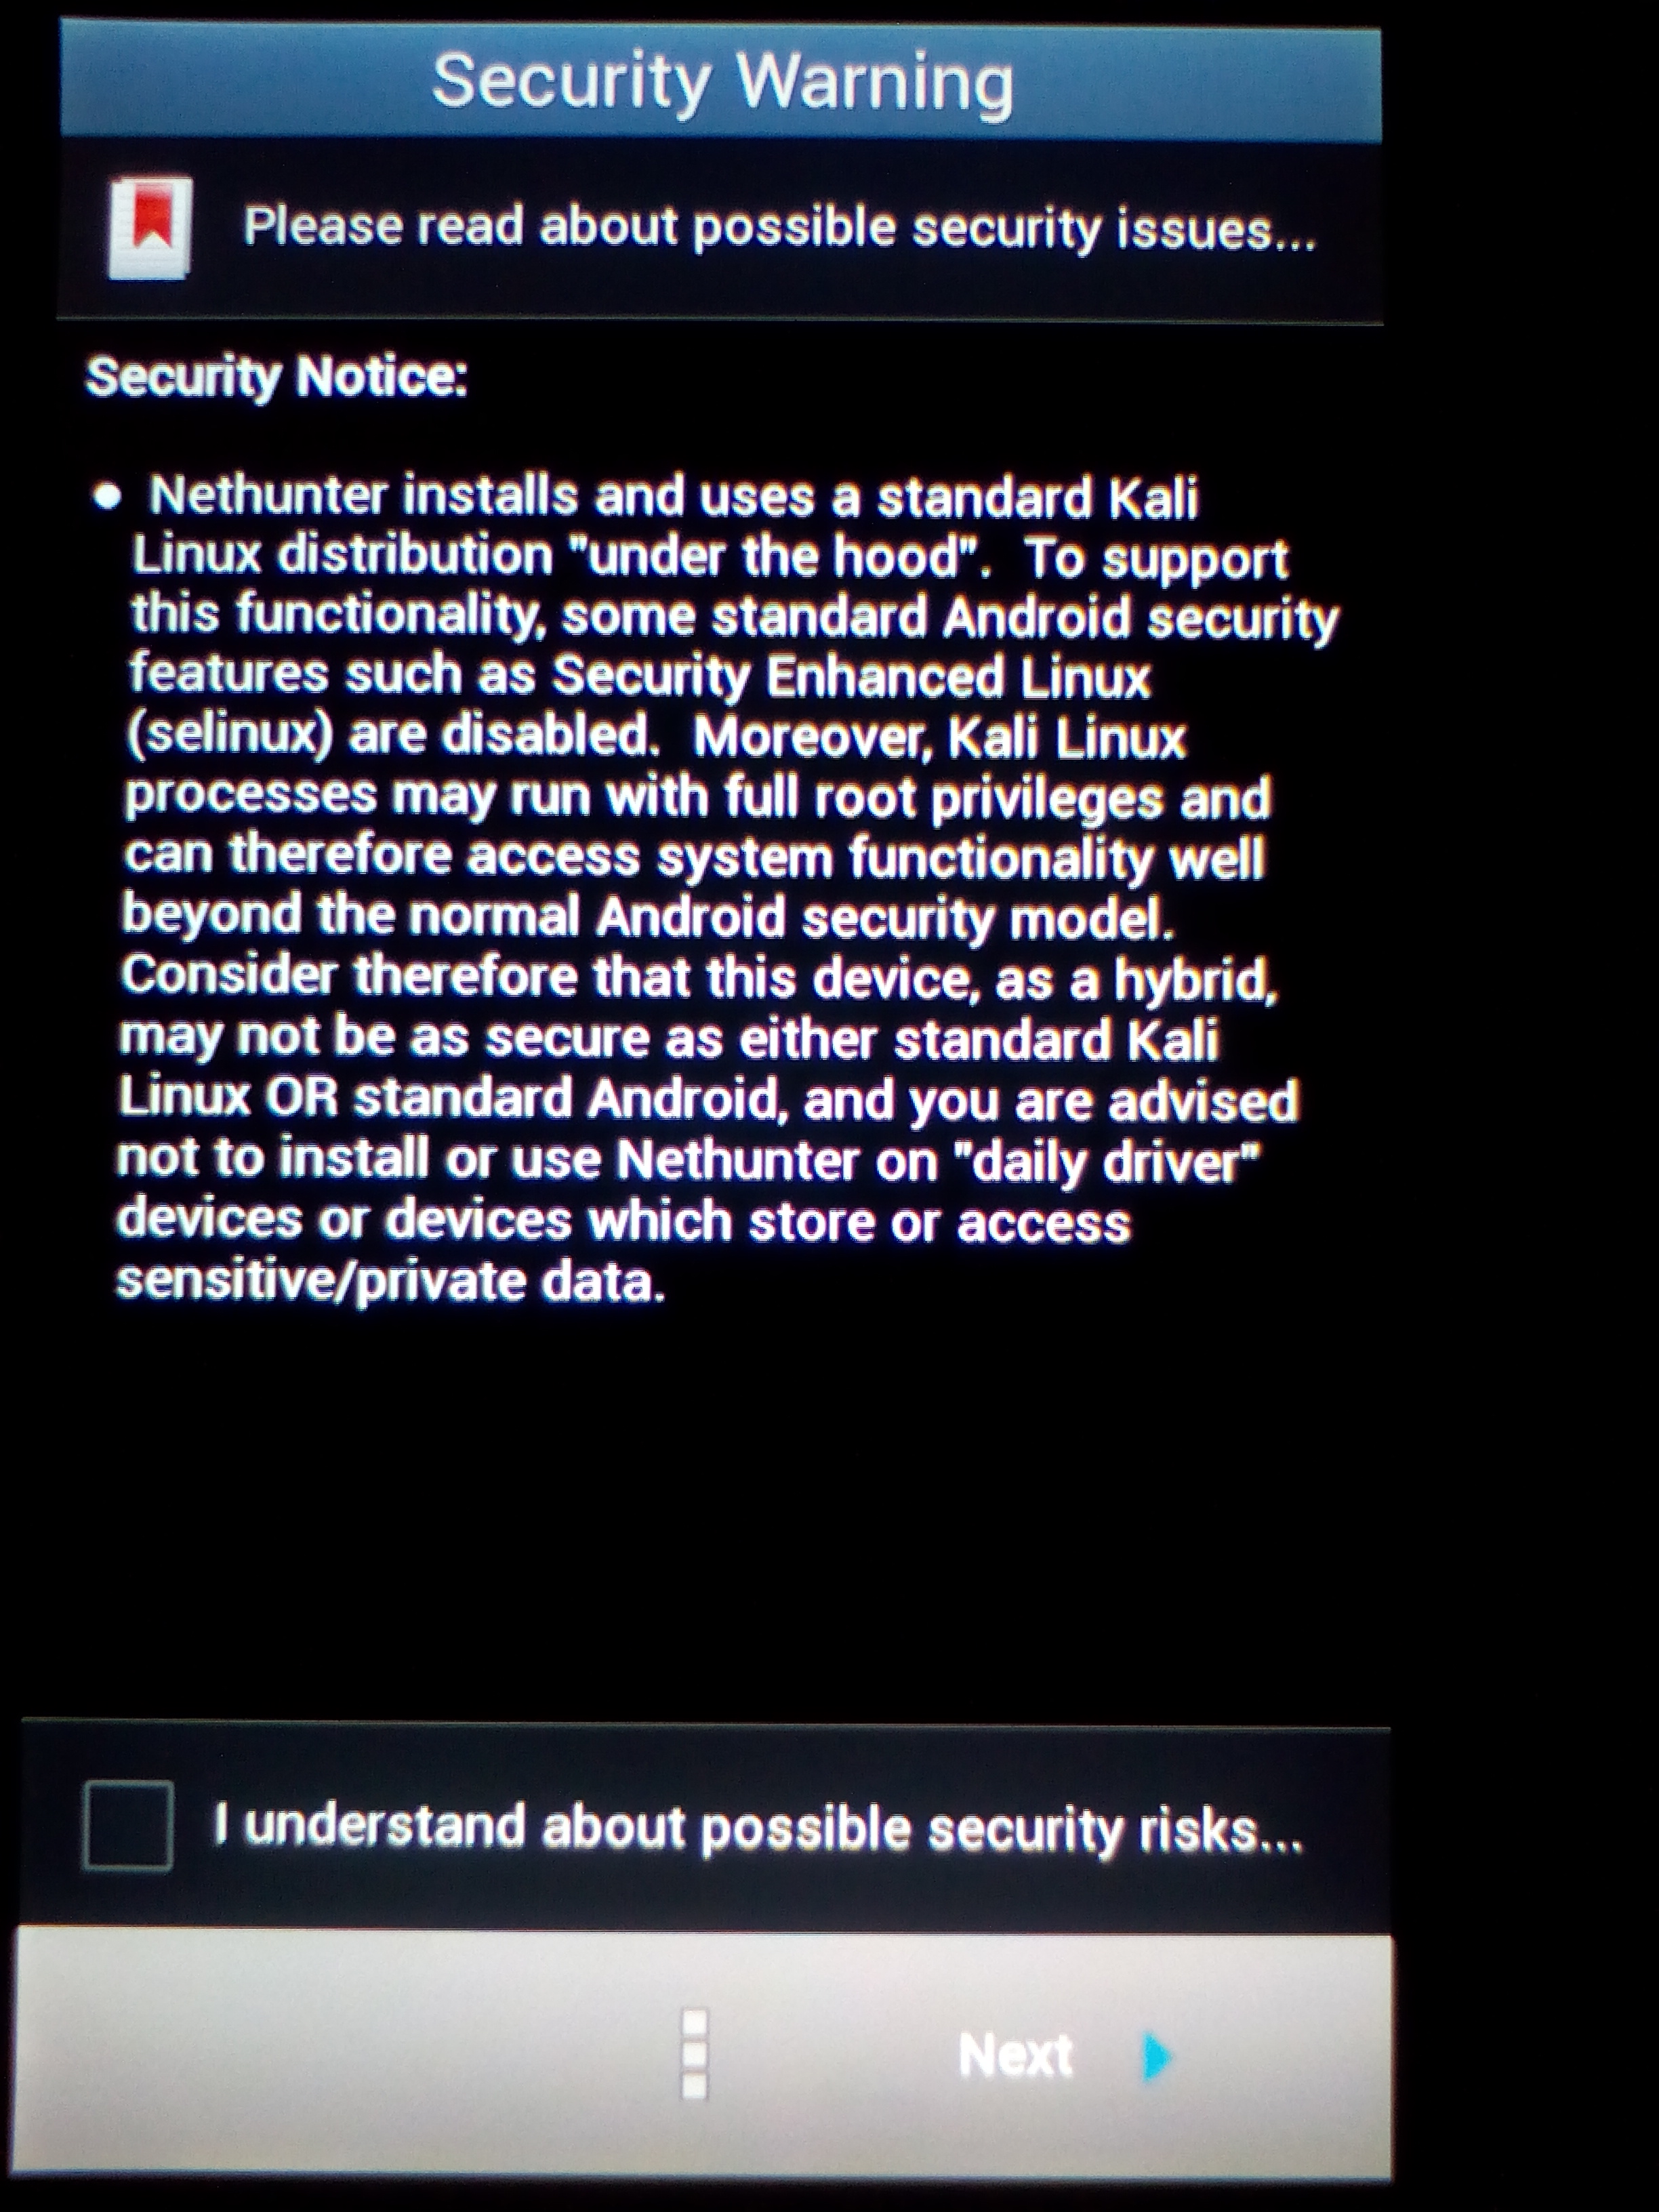
\includegraphics[scale=0.09]{./Image/img14} \\ \\
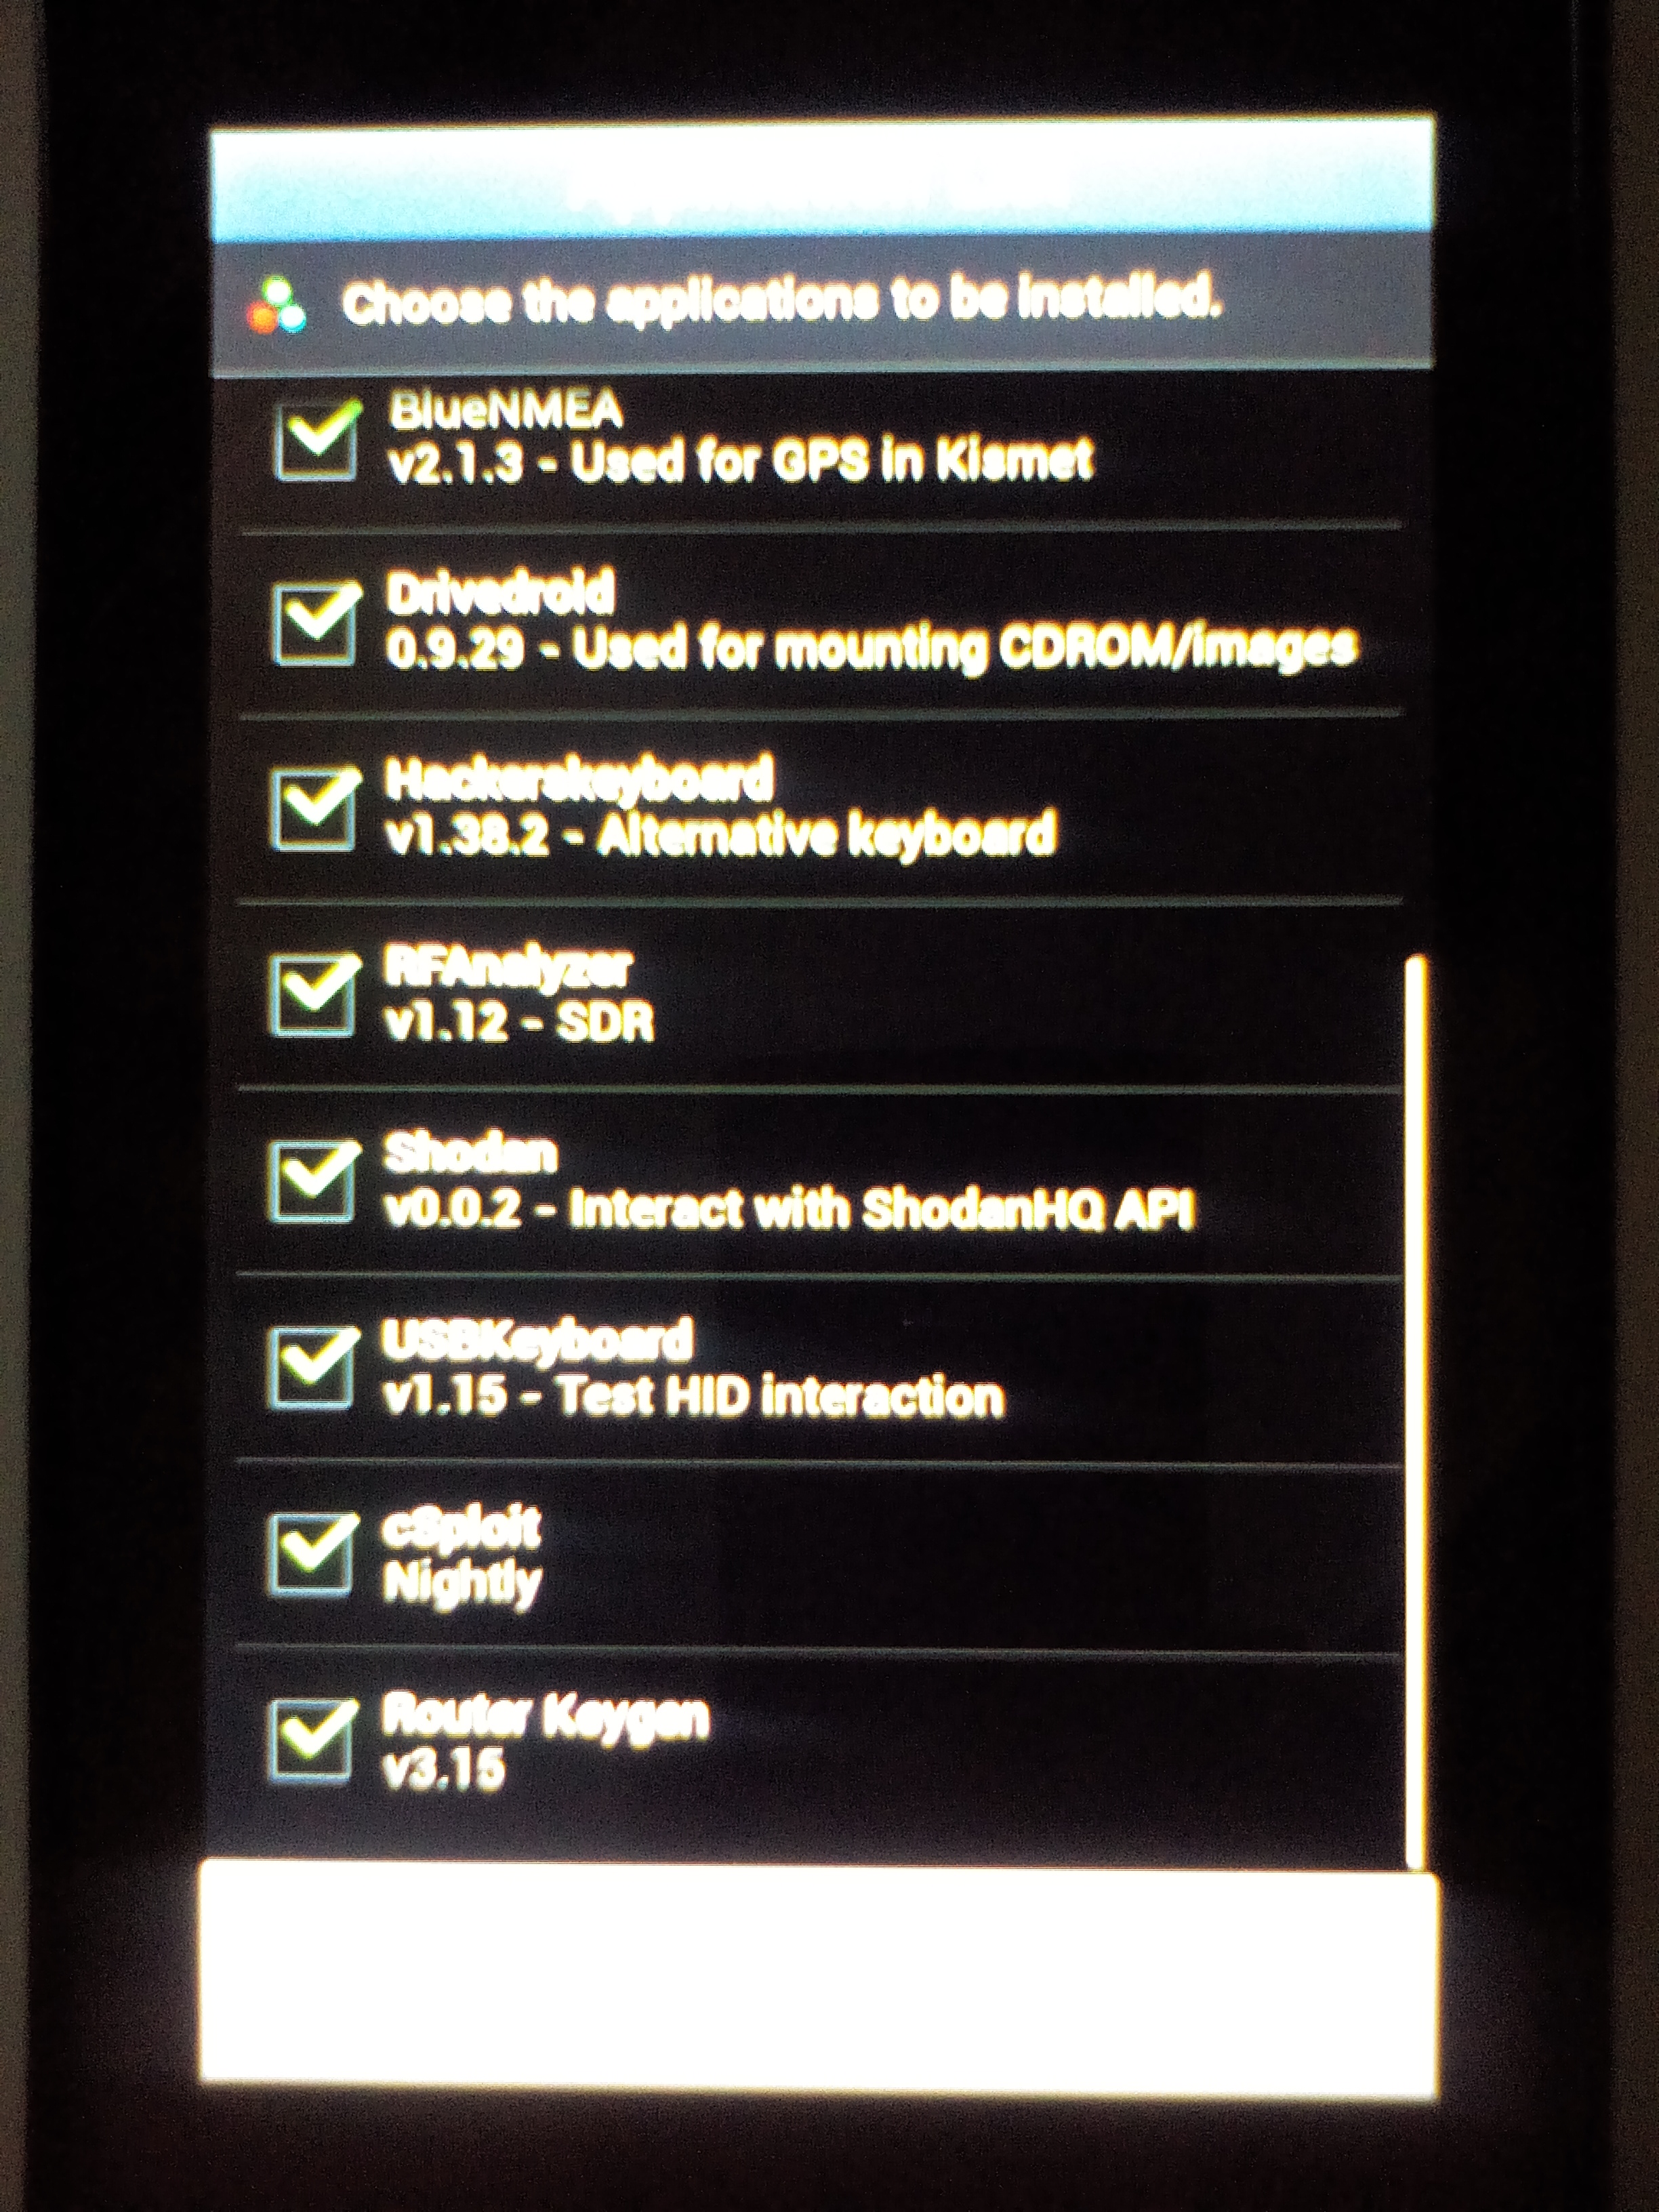
\includegraphics[scale=0.09]{./Image/img15} \\ \\
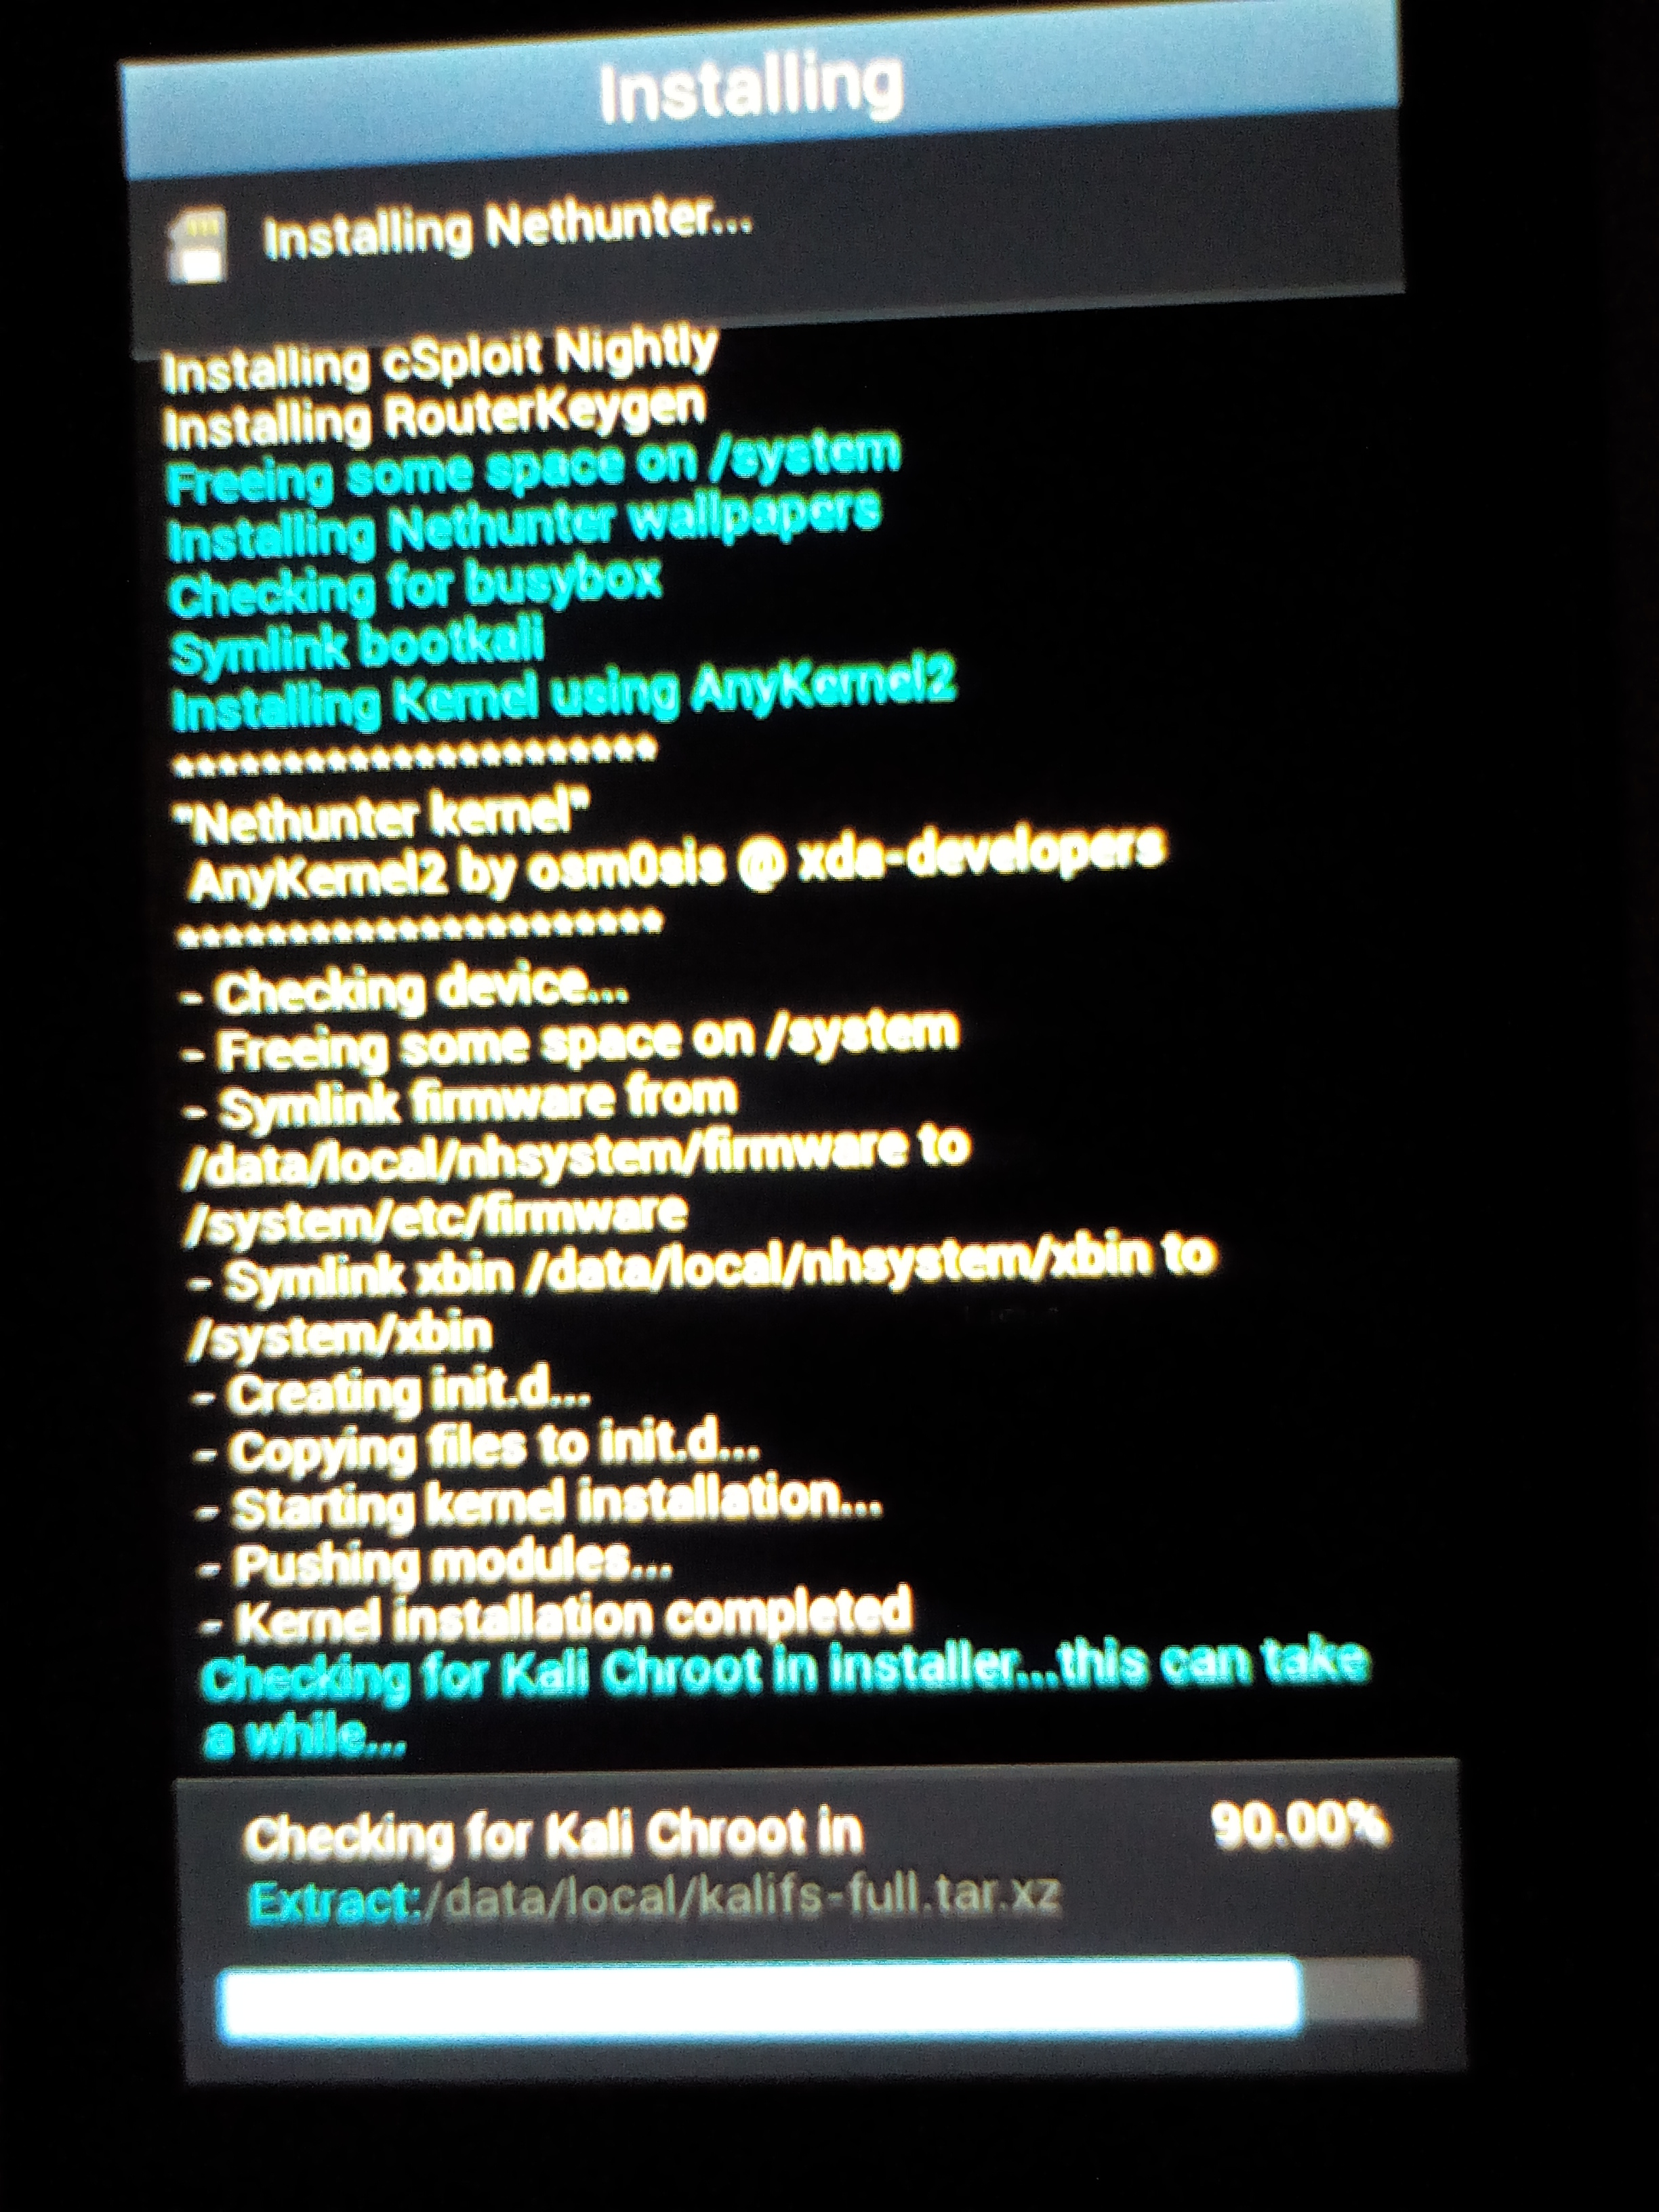
\includegraphics[scale=0.09]{./Image/img16} \\ \\
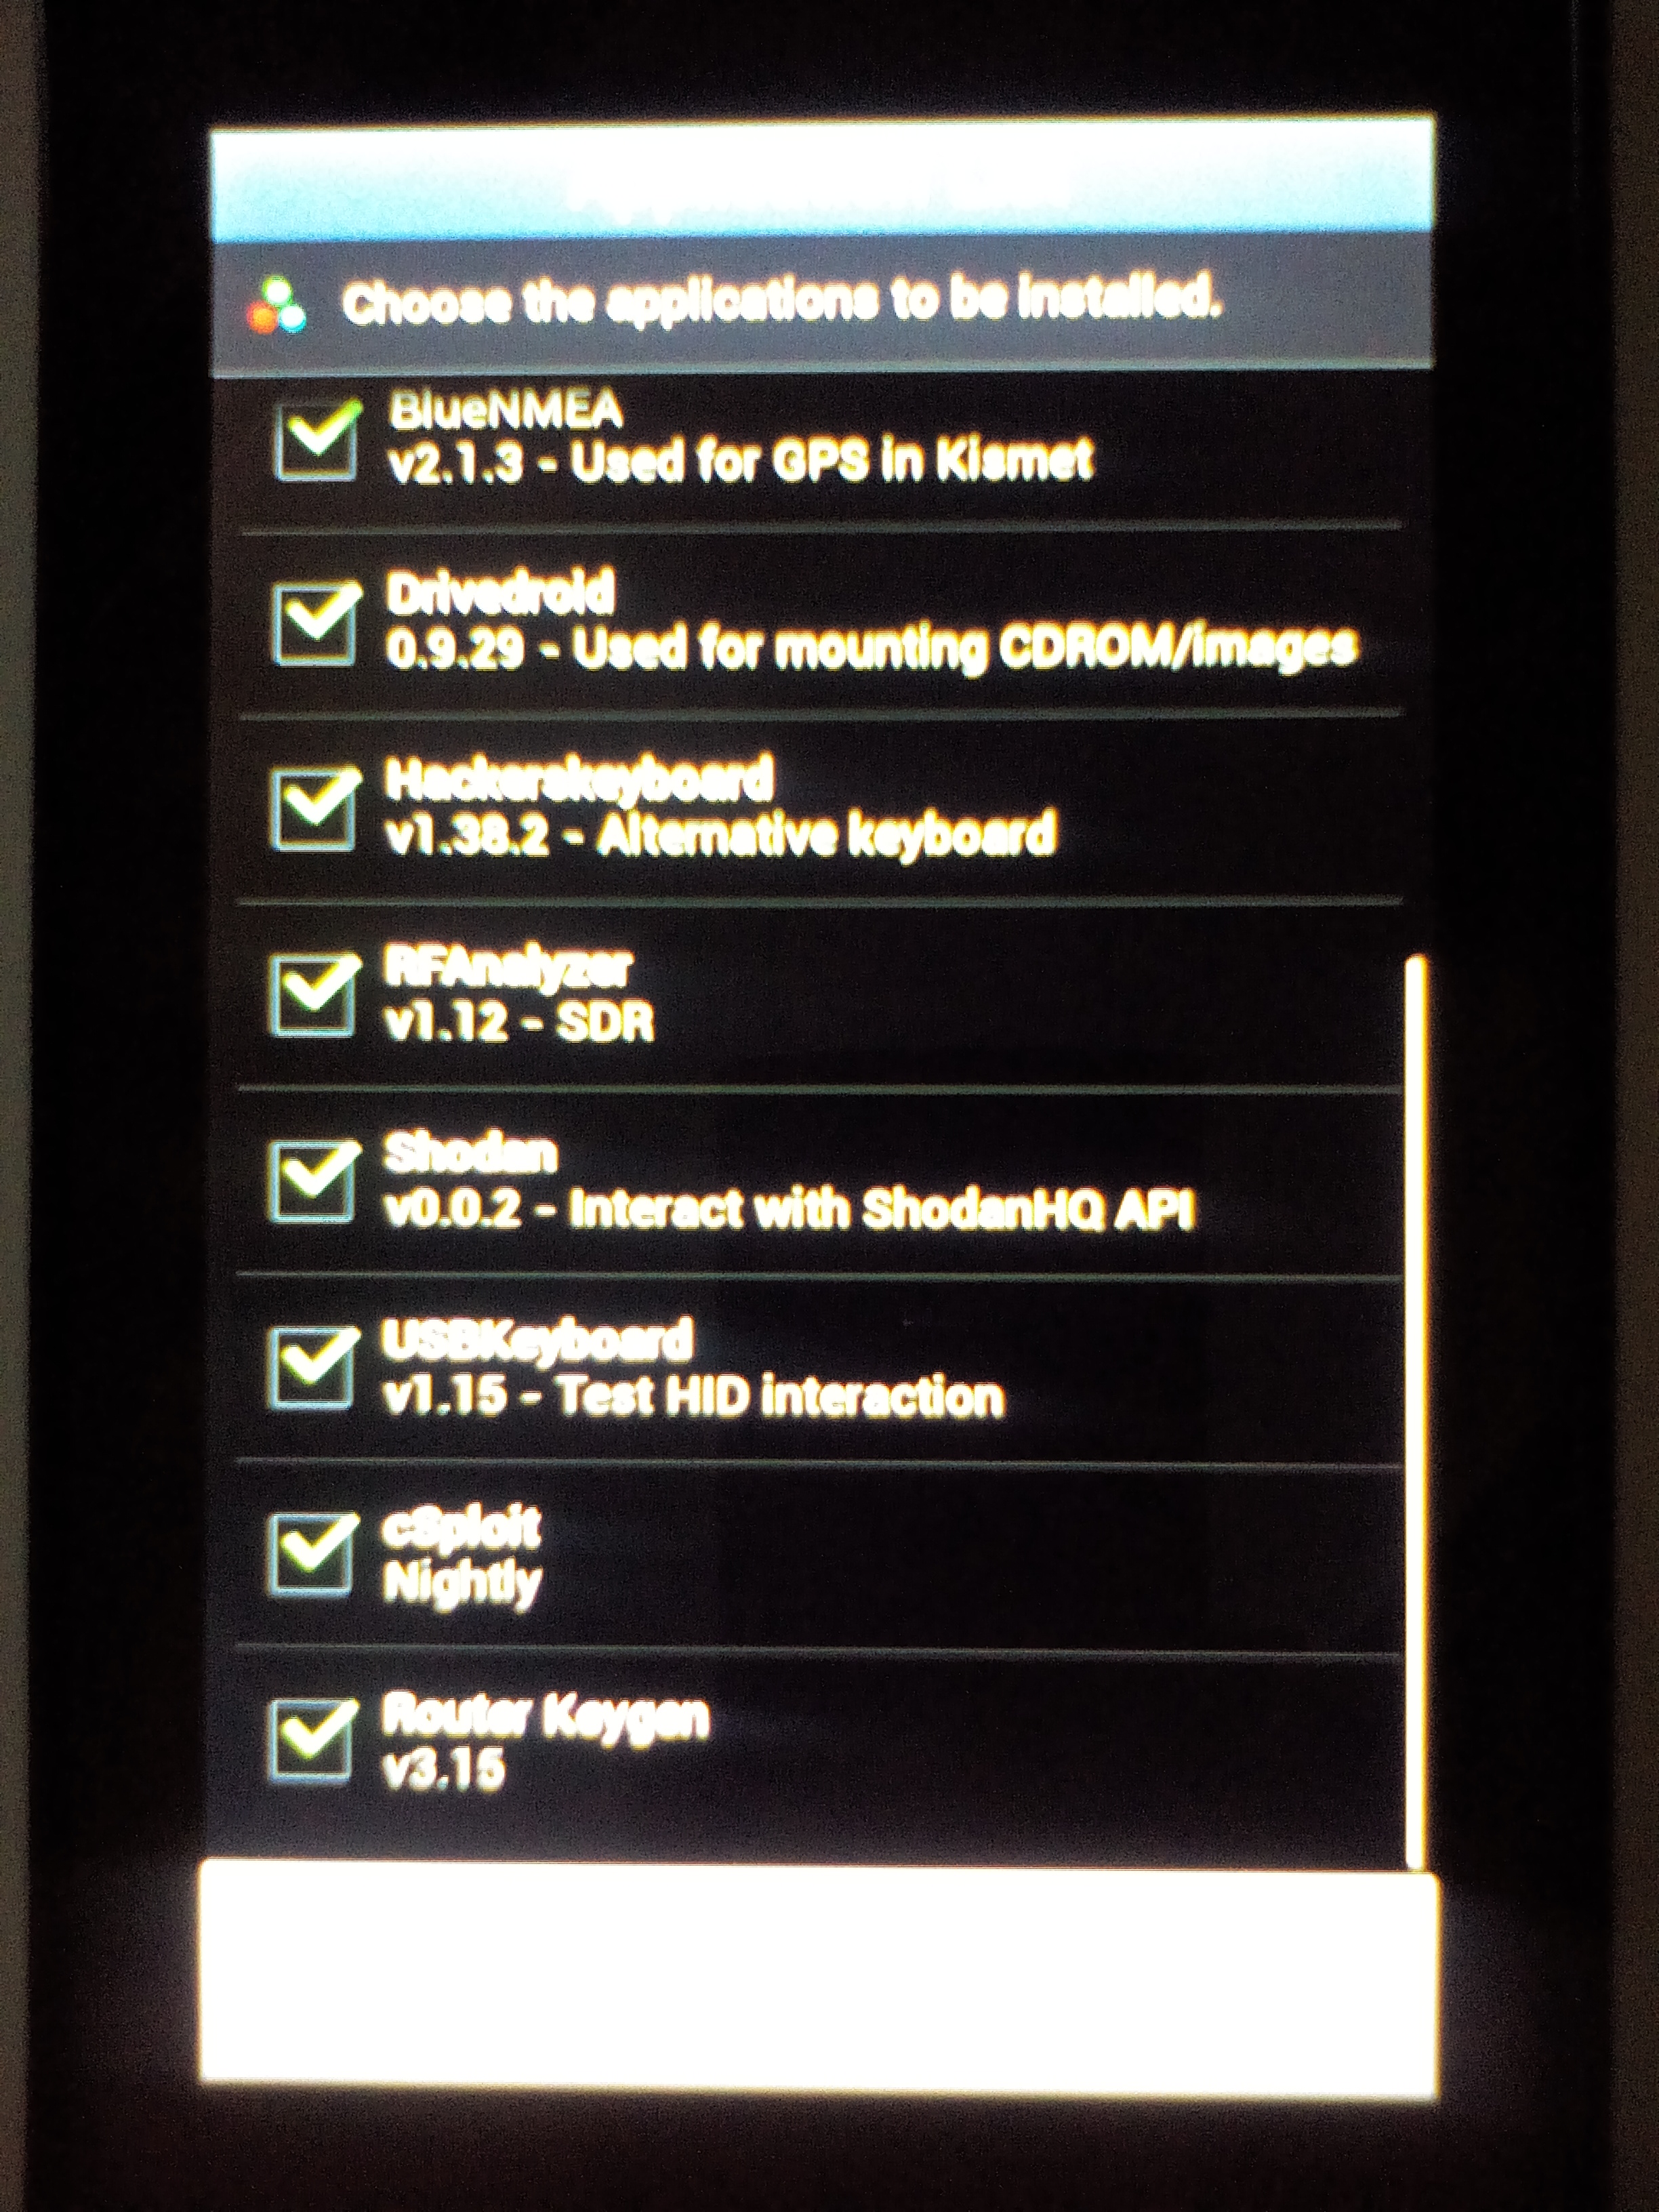
\includegraphics[scale=0.09]{./Image/img17} \\ \\
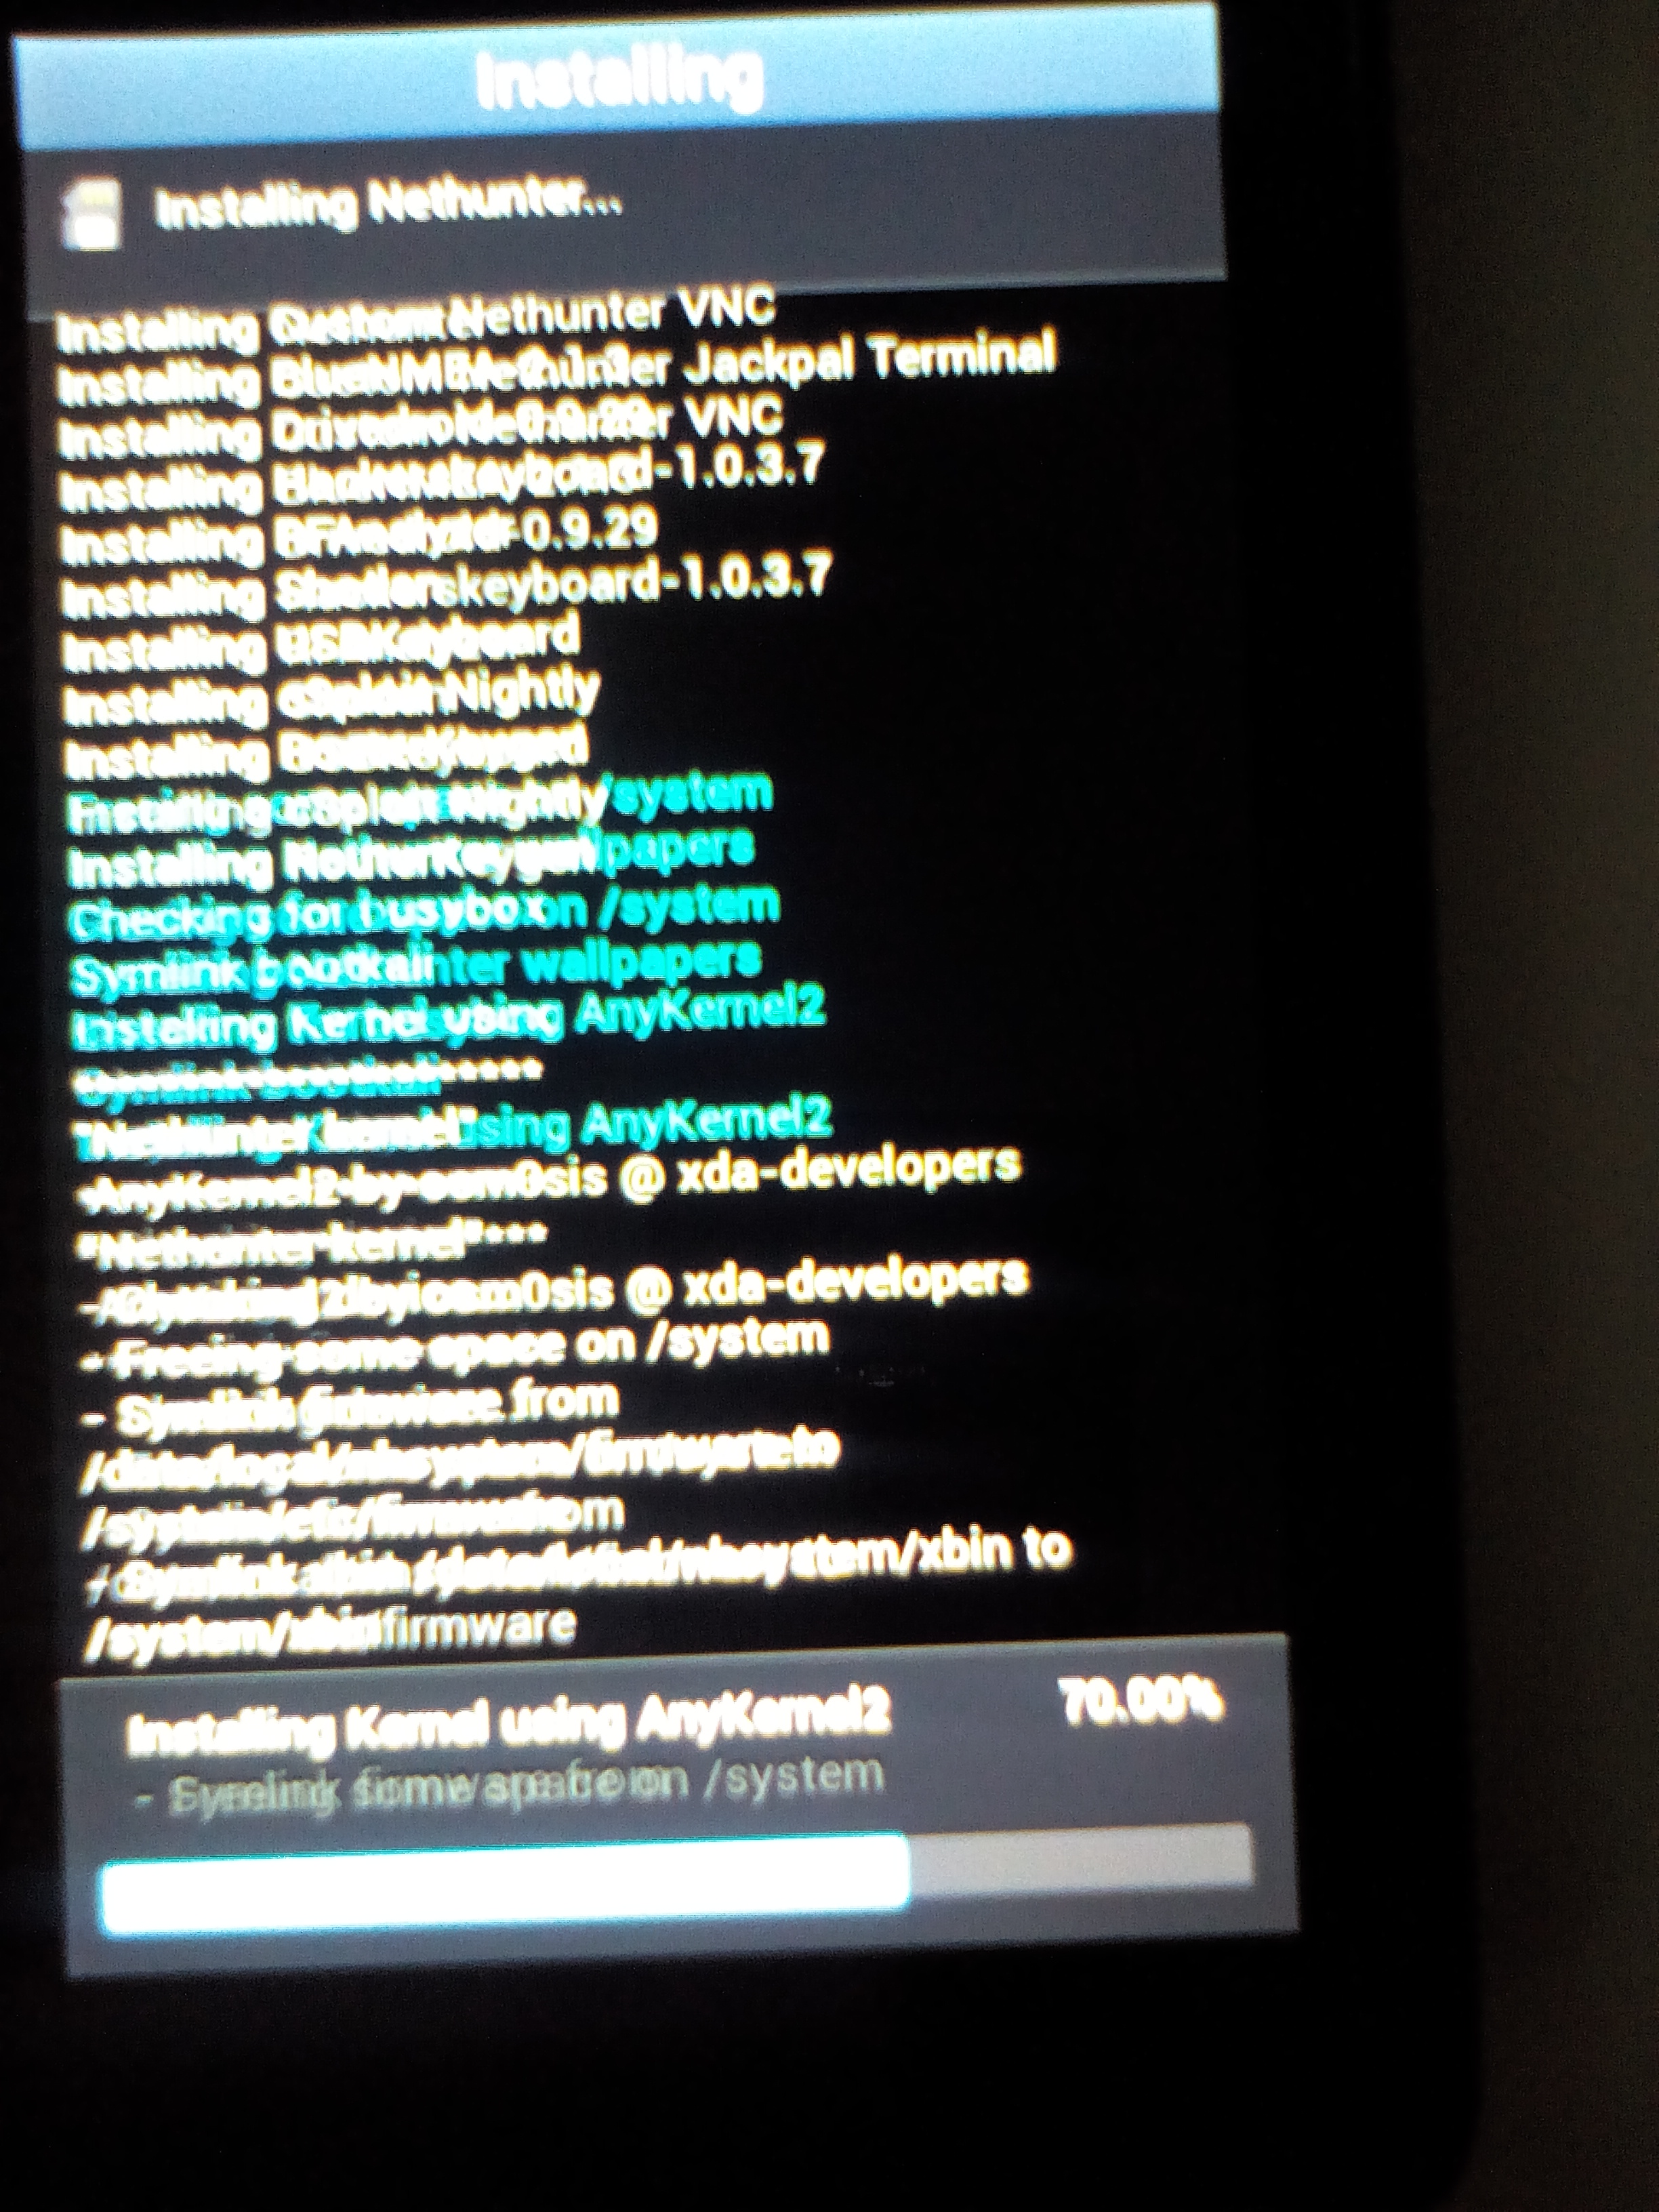
\includegraphics[scale=0.09]{./Image/img18} \\ \\
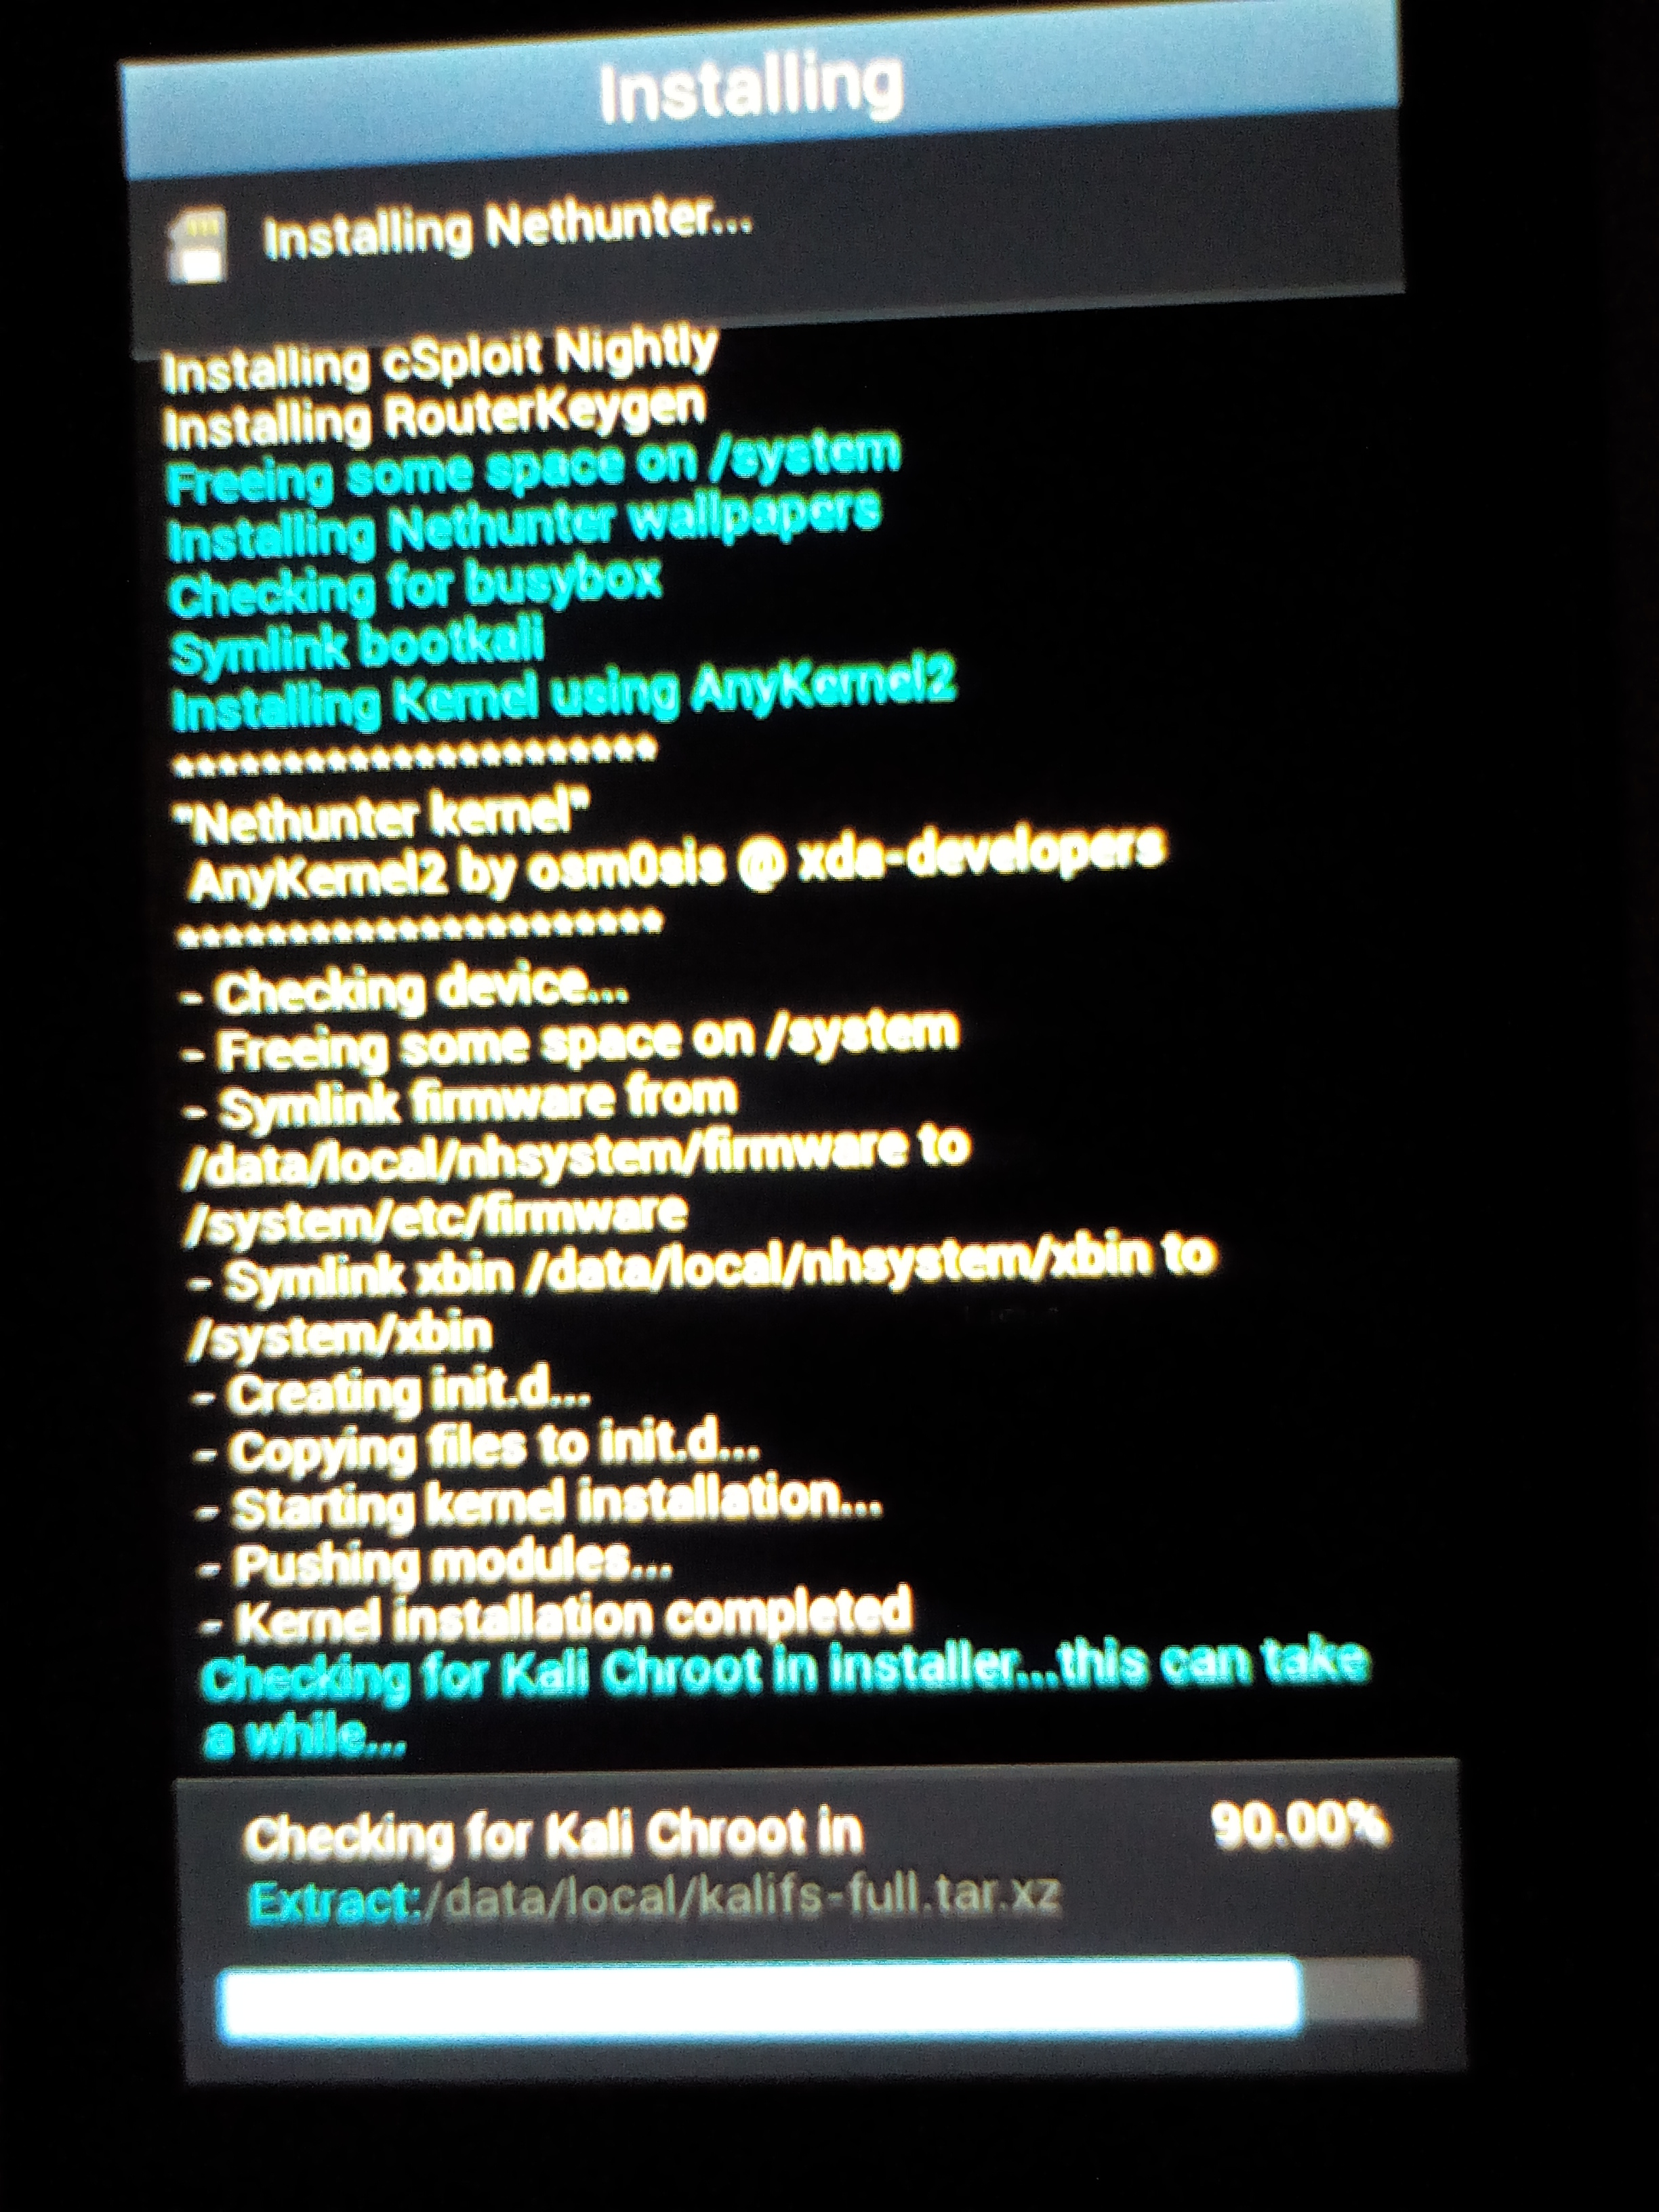
\includegraphics[scale=0.09]{./Image/img19} \\ \\


Literatur: http://www.beartechnology.com/Blog/Post/2/Kali-NetHunter-3-0-Installed-on-Nexus-7-(2012)-5-1-1-Lollipop


\end{document}